\documentclass[11pt, a4paper]{report}
\usepackage[utf8x]{inputenc}
\usepackage{ucs}
\usepackage{float}
\usepackage{array}
\usepackage{amsmath}
\usepackage{amssymb}
\usepackage{amsfonts}
\usepackage{latexsym}
\usepackage{graphicx}
\usepackage{caption}
\usepackage{ifpdf}
\usepackage{url}
\usepackage{xtab}
\usepackage{geometry}
\usepackage{longtable}
\usepackage[hidelinks]{hyperref}
\usepackage[english]{babel}
\usepackage[parfill]{parskip}
\usepackage{alltt}
\usepackage{pdfpages}

\usepackage{titlesec}

\titleformat{\chapter}{\normalfont\huge}{\thechapter.}{20pt}{\huge}

\newcommand{\comment}[1]{} \comment{This is a block comment wrapped in curly
brackets}
\begin{document}
\pagenumbering{blob}
\begin{titlepage}
\begin{center}
{\Huge {\bf Eksperter i team}}
\par
\vspace{0.1in}
{\LARGE TDT4850 - IT for en bedre verden}
\par
{\LARGE Prosjektrapport - Gruppe 2}
\par

\vspace{0.35in}

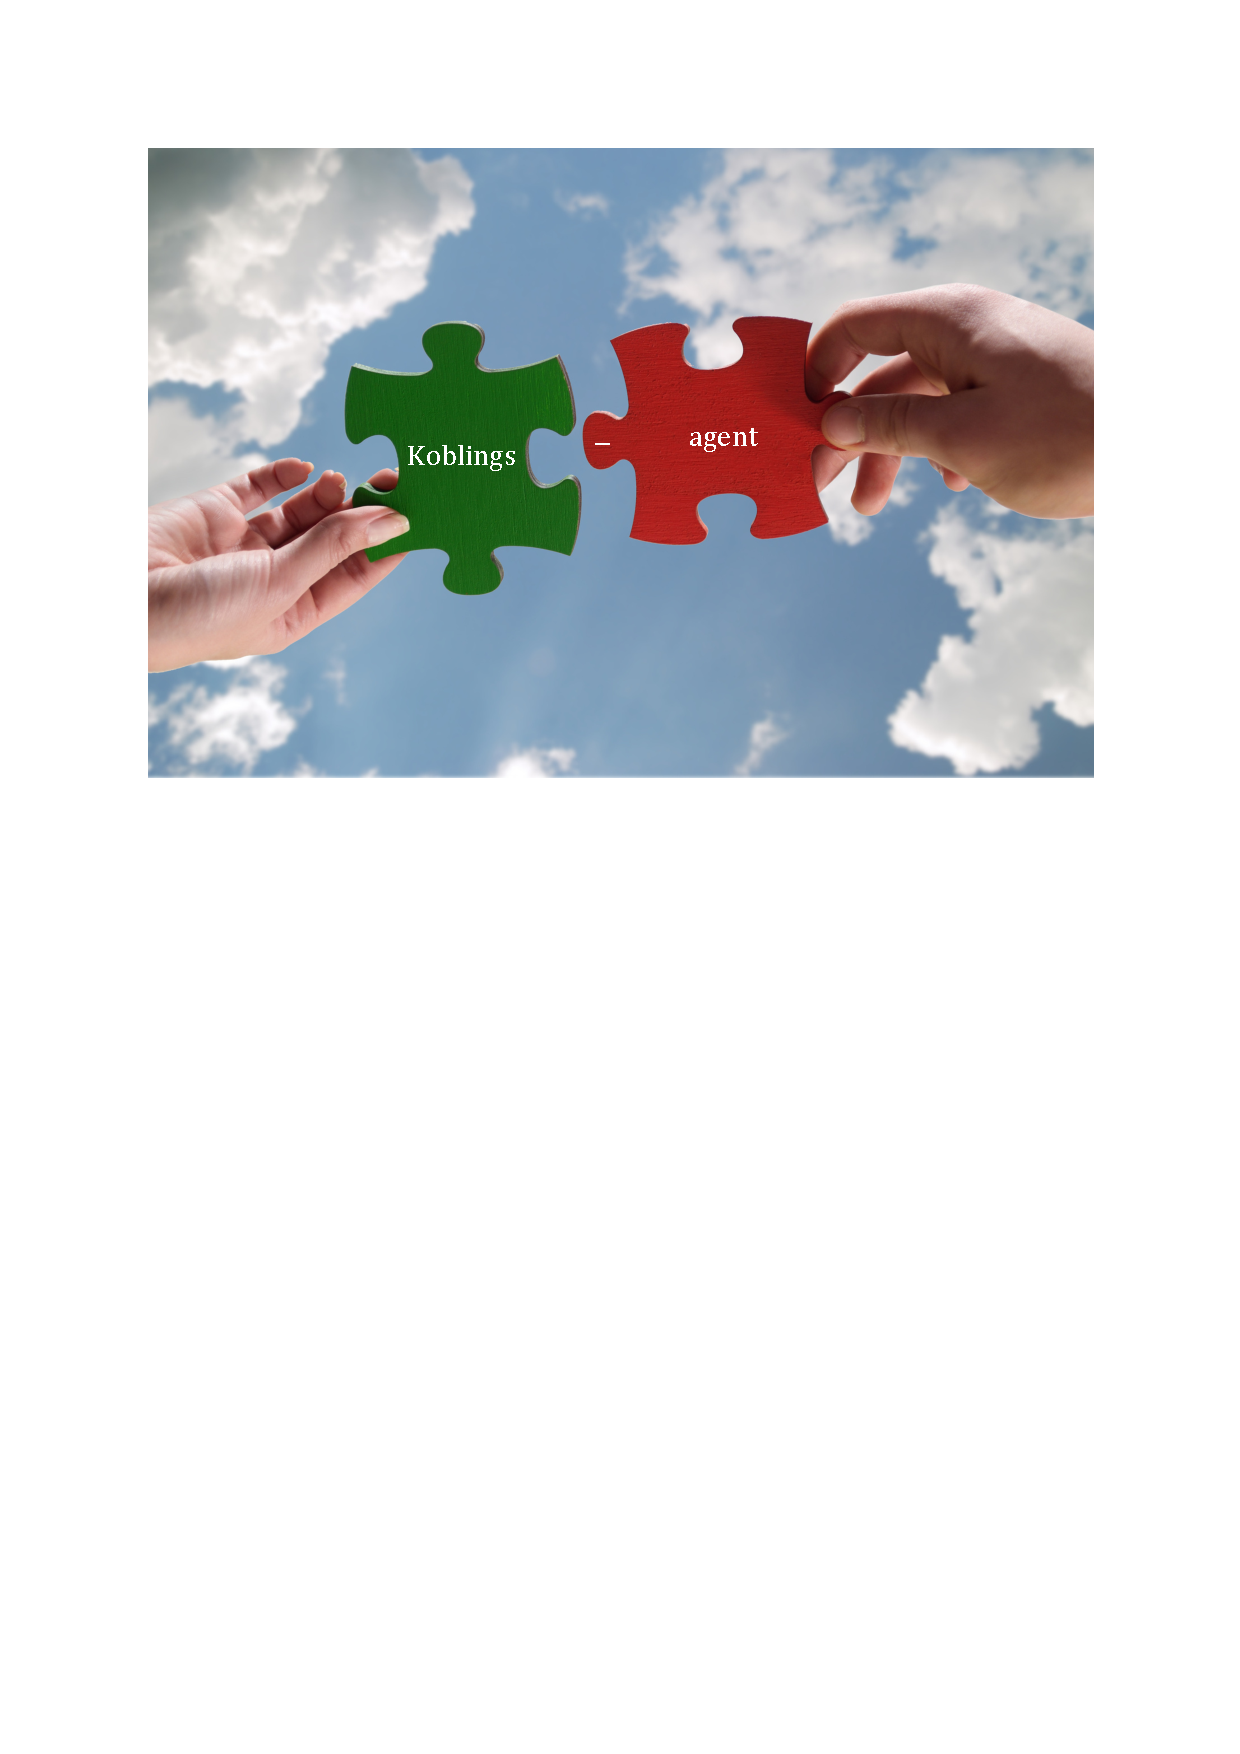
\includegraphics[scale=1.05, trim=3.5cm 19cm 0cm 1cm]{Prosjektforside.pdf}

\par

\vfill{}
\vspace{0.65in}
Espen Andreassen, Silje Mauseth, Per Bachmann, Mats Jørgensen \& Linn Vikre
\par
Vår 2014
\end{center}
\end{titlepage}

\pagenumbering{Roman}
\section*{Sammendrag}

Denne prosessrapporten er utarbeidet som en del av faget ``Eksperter i team - IT for en bedre verden'' (TDT4850) ved Norges teknisk-naturvitenskapelige universitet (NTNU). Prosessrapporten skal ta for seg ulike aspekter ved samarbeid i gruppa der mye fokus ligger på å identifisere spesifikke situasjoner som har oppstått i løpet av prosjektfasen, og trekke disse opp mot relevant teori. Det hele starter med en presentasjon av gruppesammensetningen der ulikheter og likheter blir trukket fram. Samarbeidsavtalen og ulike samarbeidsverktøy blir også presentert.\\

Videre kommer hovedkapittelet som omhandler gruppedynamikk. Her blir tre fremtredende aspekter ved gruppearbeid diskutert, henholdsvis enighet, involvering og beslutningstaking. Disse er basert på spesifikke hendelser i løpet av prosjektets gang. Kapittelet tar også for seg to spørreundersøkelser som ble utført og besvart av gruppemedlemmene under prosjektet, og vedlagt er disse undersøkelsene oppsummert i to samarbeidsindikatorer. Etter dette blir gruppetyper diskutert hvor vår gruppe blir kategorisert som en “effektiv gruppe”. Kapittelet avrundes ved å se på gruppas utvikling i løpet av prosjektet ved hjelp av Tuckmans gruppeutviklingsmodell.\\

I kapittel fire blir den personlige utviklingen til de ulike medlemmene tatt for seg i et læringsperspektiv. Her kommer de ulike medlemmene med sine tanker, og det blir konkludert med at medlemmene har hatt en positiv opplevelse av EiT og at de har blitt mer bevisste på aspekter ved gruppearbeid. Rapporten avrundes så med et evaluerings- og oppsummeringskapittel.\\

Vi vil gjerne benytte anledningen til å takke både Asbjørn Thomassen (landsbyleder) og Marianne Danielsen (daglig leder i Engasjert Byrå), samt landsbyfasilitatorene for hjelp i løpet av hele prosjektfasen.

\newpage

\tableofcontents
\listoftables
\listoffigures
\newpage

\pagenumbering{arabic}
\chapter{Innledning}
\section{Introduksjon}

``Eksperter i team'' er et obligatorisk fag for alle 4. klassinger ved NTNU. Formålet med faget er først og fremst å forbedre studentenes evne til samarbeid på tvers av fagområder. Alle studentene velger en landsby med et spesifikt tema. Teamene innad i en landsby settes sammen av landsbyleder med et mål om størst mulig tverrfaglighet. Vårt team består av studenter fra Datateknikk, Informatikk, Kommunikasjonsteknologi og Industriell Økonomi og Teknologiledelse og tilhører landsbyen: ``IT for en bedre verden''.\\

Resultatet av prosjektet er både en prosjekt- og prosessrapport. Prosessrapporten omhandler teamets samarbeid mens prosjektrapporten presenterer våre ideer i forbindelse med vår spesifikke problemstilling. Vi har valgt å se på potensialet i forbindelse med en koblingsagent som skaper koblinger mellom to parter, først og fremst med utgangspunkt i ``Gi bort dagen''. Vår problemstilling lyder som følger:
Hvilket potensiale ligger i en koblingsagent i forhold til ``Gi bort dagen'' og ``Good Stuff''?

\begin{itemize}
  \item Hva vil en koblingsagent ha å si for Good Stuffs bærekraftighet?
  \item Kan en slik koblingsagent demonstreres ved hjelp av en prototype basert på enkel koblingslogikk?
  \item Hvilke fremtidige bruksmuligheter ligger i en koblingsagent på generelt basis?
\end{itemize}

Denne problemstillingen utgjør hovedfokus for innholdet i denne prosjektrapporten, og mye av prosjektarbeidet har blitt benyttet til å utvikle en prototype på en automatisk koblingsagent. Dette har resultert i at mye tid utover rapportskriving har gått med på koding til prototypen, samt å sette seg inn i ny teknologi og nye verktøy.

\subsection{Bakgrunn for oppgaven}

Landsbytemaet: ``IT for en bedre verden'' er et åpent tema som gir mye rom for individuelle tolkninger. Som inspirasjon i forbindelse med utarbeidelsen av en problemstilling holdt Marianne Danielsen, daglig leder for Engasjert Byrå, en presentasjon om ``Gi bort dagen''. Konseptet ``Gi bort dagen'' skal motivere ressurssterke bedrifter og organisasjoner til å ``gi bort en dag'' ved å knytte relasjoner med mindre ressurssterke organisasjoner som trenger hjelp av ulikt slag.

Konseptet har vært vellykket og antall relasjoner mellom mottakere og givere har økt jevnt siden oppstarten i 2012. Da antall relasjoner øker årlig kreves det stadig mer ressurser i forbindelse med relasjonsbyggingen siden dette foregår manuelt i dag. Marianne har planer om å kunne videreutvikle ``Gi bort dagen'' ved å grunnlegge det ideelle selskapet ``Good Stuff'' i nær fremtid. ``Good Stuff'' vil være prosjekteier for ``Gi bort dagen''. ``Good Stuff'' skal være bærekraftig ved blant annet å tilby etisk/moralsk rådgivning og konferanser. For å oppnå dette vil det være svært gunstig med teknologi som forenkler prosessen med å koble en giver og en mottaker. Dagens opplegg med manuelle koblinger mellom mottakere og givere vil være alt for tid-og ressurskrevende dersom ideen skal utvikles videre. I den forbindelse har vi valgt å se på mulighetene en automatisk koblingsagent vil tilføre ``Gi bort dagen'' i fremtiden. I hvilken grad kan en automatisk koblingsagent bidra til at ``Gi bort dagen''-prosjektet blir mer skalerbart, og samtidig bærerkraftig? I tillegg ønsker vi å se på hvilke andre bruksområder innen frivillighet som en automatisk koblingsagent kan benyttes til.

\subsection{Motivasjon}

Gruppas medlemmer hadde tilsynelatende ganske like forventninger til prosjektet. Vi forventet alle å utvikle oss selv, og da spesielt med tanke på samarbeidsevner. Et felles ønske var at vi ved prosjektslutt skulle ha bedre innsikt i hvordan man bør forholde seg til en gruppe for å oppnå en optimal prosess med et best mulig resultat. I tillegg hadde vi et ønske om å tilegne oss ny kunnskap ved utvikling av, og arbeid med koblingsagenten. Et generelt mål var å kunne utnytte hverandres tverrfaglighet til å få innsyn i fagområder vi i utgangspunktet hadde mindre innsikt i.

Landsbytemaet ``IT for en bedre verden'' er implisitt en motivasjon. Det å kunne være med å utvikle noe som resulterer i en bedre verden, er noe som både inspirerte og motiverte oss. Å bidra til at vanskeligstilte og mindre ressurssterke parter får hjelp, tilfører prosjektet en ekstra dimensjon som gir deg følelsen av å være med på noe som er større enn deg selv.

\subsection{Begrensninger}

Den største utfordringen og begrensningen i prosjektet var mest sannsynlig tidsaspektet. Til sammen er det satt opp 15 landsbydager med arbeidstid på åtte timer per dag. Deler av disse dagene vil dog bli benyttet til andre øvelser, noe som fører til mindre avsatt arbeidstid til selve prosjektet. Dette er en av begrunnelsene for å utvikle en prototype istedenfor et fullstendig system. Samtidig skal arbeidet reflektere over muligheter og resultater et fullstendig system kan føre med seg ved et videre arbeid.

Videre kan kompleksitet bli et problem i prosjektet. I sammenheng med tidsaspektet diskutert over må begrensninger foretas for å kunne overkomme begge utfordringene. Noe som vil gjenspeile seg i prototypen.

Som det fremgår i introduksjonen består gruppen av personer med relativt like bakgrunner. I et prosjekt kan det ofte være fordelaktig med tverrfaglige medlemmer for å forsikre et høyt kunnskaps- og erfaringsnivå. Det er viktig at gruppa er observant på dette faktum, og baserer prosjektet på de kunnskapene og erfaringene vi besitter, men samtidig utfordrer oss selv for å unngå fenomenet gruppetenkning. Gruppetenkning er ofte et resultat av gruppemedlemmer med like interesser, egenskaper og kunnskaper, og kan føre til at første og antatt beste løsning blir valgt (Wheelan, 2009)\citep{effectiveTeams}.

\subsection{Disposisjon}

I denne rapporten vil vi først presentere forarbeidet som er gjort i forbindelse med prosjektet i kapittel 3. Dette arbeidet besto blant annet av brainstorming, presentasjon og møte med Marianne Danielsen og observasjon av data, og bidro til at vi fikk et klarere bilde av krav og spesifikasjoner. Videre inneholder del 3 teori om agenter for å etablere en felles forståelse av begrepet. Delen inneholder mer spesifikke definisjoner, kategorisering og typiske egenskaper ved agenter. Deretter beskriver vi prototypen til koblingsagenten i del 4, hvordan den overordnede koblingsprosessen foregår fra brukerens perspektiv, men også hvordan den underliggende koblingslogikken fungerer. Kapittel 5 er diskusjon rundt koblingsagentens påvirkning på Good Stuff, i tillegg til videre bruksmuligheter for en generell koblingsagent. Rapporten avsluttes med resultater av en koblingagent (\ref{chapter:forslag}), konklusjon (\ref{chapter:konklusjon}) og videre arbeid (\ref{chapter:viderearbeid}).


\chapter{Rammeverk for gruppearbeid}
\section{Sammensetning}
\label{sec:sammensetning}
Ved oppstart ble studentene involvert i EiT-landsbyen delt inn i grupper. Disse gruppene var fordelt slik at de skulle oppnå en størst mulig tverrfaglighet. Under vil en presentasjon av hvert enkelt medlem av gruppen bli gitt i tillegg til en uttalelse fra personen om forventninger og ambisjoner i faget.
Espen er en 22 år gammel gutt fra Tromsø. Han karakterisere seg selv som utadvent, ærlig og detaljeorientert, men kan være sta i noen tilfeller. På fritiden går mye av tiden til sport, teknologi, film og musikk, samt reiser. Den faglige bakgrunnen er realfag ved videregående skole og han går for øyeblikket på Datateknologi ved NTNU med spesialisering innenfor Programvareutvikling.\\

\textit{``Mine forventninger til faget er relativt store. Noen av målene jeg ønsker å oppnå er økt kunnskap, et bra sluttprodukt, å lære mer om meg selv (min `rolle' i en arbeidsgruppe) og forhåpentligvis lære av andres kunnskaper. Jeg håper videre at EiT vil bidra til en progresjon i hvordan jeg samarbeider og forholder meg til team der medlemmene besitter ulike (faglige) bakgrunner. Dette er viktig for meg siden det er noe som er en ettertraktet egenskap i arbeidsmarkedet.''}\\

Silje er ei 23 år gammel jente fra Fetsund. Hun ser på seg selv som initiativrik, selvdisiplinert og ansvarsfull, men kan fort bli rastløs hvis ting går tregt. Til daglig er hun svært aktiv innenfor håndball. Hun har også en realfaglig bakgrunn fra videregående skole, og studerer for øyeblikket Industriell Økonomi og Teknologiledelse Datateknologi/ Kommunikasjonsteknologi med teknisk spesialisering innenfor Telematikk og hovedprofilen Strategi ved NTNU.\\

\textit{``Mine forventninger til EiT er ganske store. Jeg har hørt mye forskjellig om faget og er spent på å danne mitt eget inntrykk. Jeg tror at man kan lære mye om både seg selv og gruppearbeid dersom man er villig til å legge inn litt arbeid og engasjement. Ved å være positiv og arbeidsvillig håper jeg å kunne bli et bedre gruppemedlem ved å bli mer bevisst på hvordan mine handlinger påvirker gruppedynamikken.''}\\

Mats er en 22 år gammel gutt fra Brønnøysund. Han beskriver seg selv som pålitelig, hjelpsom og tålmodig, men føler han kan opptre som skeptisk til tider. Han liker å bruke tiden på datarelaterte ting, trene og er interessert i motorsykler. Han utførte en realfaglig utdanning ved videregående skole, og går for øyeblikket Kommunikasjonsteknologi med spesialisering innen Telematikk ved NTNU.\\

\textit{``Mine forventninger til EiT er å bli bedre til å samarbeide og kommunisere med andre i en gruppe. Jeg har litt blandede følelser overfor EiT, siden jeg har hørt mye forskjellig fra andre som har hatt faget tidligere. Samtidig er jeg spent på hvordan samarbeidet kommer til å utvikle seg i løpet av prosjektet og ser frem til et spennende semester!''}\\

Per er en 22 år gammel gutt fra Moss. Han karakteriserer seg selv som pålitelig, ydmyk og hyggelig, men føler han kan bli usikker i visse situasjoner. Til daglig har han interesse innenfor sport og teknologi. Han har som de andre medlemmene en utdanning innen realfag ved videregående skole, og har valgt retningen Datateknologi ved NTNU der han spesialiserer seg innenfor Komplekse Systemer.\\

\textit{``Mine forventninger til EiT er å lære mer om gruppearbeid der man har medlemmer med en forskjellig faglig bakgrunn. Jeg er også spent på hvordan en refleksjon av gruppearbeidet eventuelt kan forbedre et arbeid og hva jeg kan trekke ut av dette for å bli et bedre som gruppemedlem.''}\\

Linn er en 23 år gammel jente fra Bærum. Hun ser på seg selv som målrettet, lite selvhøytidelig og positiv, men kan til tider bli oppslukt i arbeidet hun har påtatt seg. På fritiden er hun meget interessert i alpint og sport generelt. Hun har en idretts- og realfaglig bakgrunn fra videregående skole, og studerer for øyeblikket Informatikk ved NTNU.\\

\textit{``Forventningene mine til EiT er litt midt på treet etter å ha hørt fra tidligere studenter hvordan de opplevde faget. Jeg håper at det skal bli lærerikt og at jeg kommer på en gruppe som klarer å arbeide godt sammen tross eventuelle konflikter eller uenigheter som kan oppstå. En annen ting jeg håper på er at vi får brukt kunnskapen vår innenfor IT til å utvikle en simpel prototype.''}\\

\section{Er gruppesammensetningen heterogen?}
\label{sec:gruppesammensetning}
Å betegne en gruppe som enten heterogen eller homogen er ofte umulig. Gruppemedlemmer er simultant heterogene og homogene pga. de hundrevis av karakteristikker og egenskaper hvert enkelt medlem besitter \citep{gruppeteori}. Kilder til ulikheter kan gjerne deles inn i tre kategorier: demografiske karakteristikker, personlige karakteristikker og evner og ferdigheter \citep{gruppeteori}. Under blir disse tre diskutert der hovedvekten ligger på de to sistnevnte kategoriene.\\

Det er verdt å legge merke til at gruppesammensetningen er veldig homogen i forhold til de demografiske karakteristikkene. Alle medlemmer tilhører den samme aldersgruppa, er født og oppvokst i Norge og kommer fra realtivt velstående familier. Den mest markante spredningene er nok den geografiske der noen kommer fra så langt nord som Tromsø, mens andre er oppvokst i Oslo og omegn. Det kan også være verdt å nevne at ingen av gruppemedlemmene er enebarn, som videre fremhever homogeniteten i denne kategorien.\\

I vår sammenheng er det som nevnt mer interessant å analysere de personlige karakteristikkene og evnene og ferdighetene de ulike medlemme besitter. Som det vil komme frem er disse to kategoriene ganske ulikt vektet i forhold til homogenitet og heterogenitet. I løpet av prosjektfasen ble det tydelig at medlemmene var ganske ulike i forhold til de personlige egenskapene. For noen var det lettere å ta ordet i diskusjoner enn for andre . Vi så et skille mellom ekstroverte og introverte personer. Dette var noe som derfor ble et viktig fokus for gruppa å ta hensyn til slik at alle medlemmene ble involvert i omtrent lik grad.\\

I oppstartsfasen ble vi fort observante på at medlemmene kom fra ganske like faglige bakgrunner. Alle hadde gjennomgått en realfaglig utdanning ved videregående skole. Videre var spredningen i retningene ved NTNU ikke så stor. Representert var Informatikk, Industriell Økonomi og Teknologiledelse Datateknologi/Kommunikasjonsteknologi, Datateknologi og Kommunikasjonsteknologi. Alle disse sentrerer seg rundt mye av det samme. Det er selvfølgelig noen ulikheter, men det er greit å konkludere med at vi har relativt homogene evner og ferdigheter hvis vi ser på det hele i et overordnet perspektiv.\\

Som det kommer frem fra teksten over er det ikke lett å trekke slutning med at gruppen enten er homogen eller heterogen. Gruppa er nokså homogen på det faglige, men noen er tydelig mer ekstroverte enn andre. I løpet av prosjektet var det viktig at vi rettet blikket mot å utnytte både de heterogene og homogene kvalitetene gruppa besatt. Et sitat fremhever viktigheten av å utnytte mulighetene av ulikheter i dagens samfunn:``Diversity among members is no longer exceptional or optional, it is the everyday rule.'' \citep{gruppeteori}.\\

\section{Samarbeidsavtalen}
På et tidlig stadium ble en samarbeidsavtale utarbeidet i felleskap innad i gruppa (se Appendix \ref{appendix:samarbeidsavtale}). Hensikten med en slik kontrakt er å klargjøre spillereglene for samarbeid i løpet av et prosjekt eller arbeid. Det er viktig at avtalen er konkret og at alle medlemmer har samme forståelse for punktene de samtykker med for å ikke skape misforståelser. Moderne forskning viser at det gjerne er tre punkter som er sentrale for å oppnå et effektivt team: leveranse, trivsel og læring (Hjertø, 2008). Dette er illustert i Teamtrekanten i figur \ref{fig:kompetansetrekant} som viser den gjensidige avhengigheten mellom punktene.\\

\begin{center}
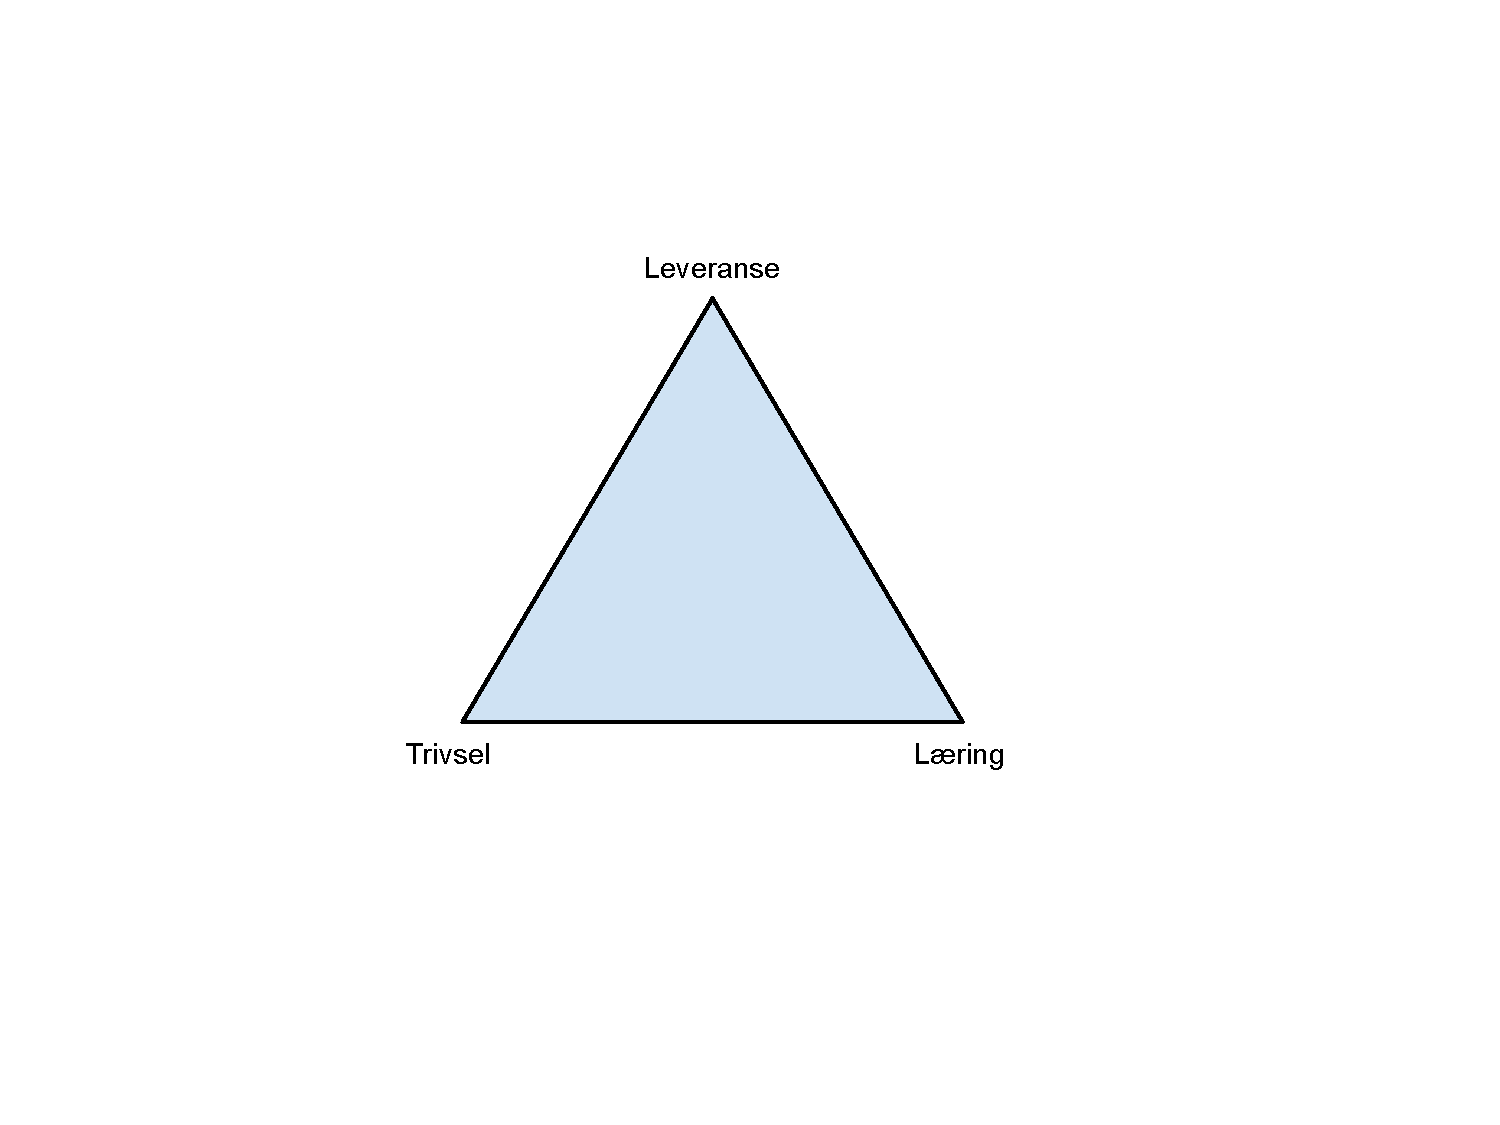
\includegraphics[clip=true, width=1 \textwidth,
trim=0cm 5cm 0cm 3cm]{kompetansetrekant.pdf}
\captionof{figure}{Kompetansetrekant}
\label{fig:kompetansetrekant}
\end{center}

Det ble i den grunn naturlig for oss å ta utgangspunkt i disse tre punktene når samarbeidsavtalen ble produsert. I punktet relatert til leveranse har vi fremhevet behovet for at de ulike gruppemedlemmene er bevisste på å ta ansvar for arbeid de utfører, og at dette arbeidet tilfredsstiller kravet om kvalitet som gruppa har blitt enig om. Et annet fokus innenfor leveranse har vært punktlighet og opprettholdelse av tidsfrister. Under trivsel har hovedfokuset blitt satt på inkludering. I tillegg har det vært viktig å være observante på eventuelle konflikter, og ta tak i disse på et tidlig tidspunkt før de eskalerer til et problem. Innenfor punktet læring har blikket blitt rettet mot deling av kunnskap. Det er viktig at medlemmene blir holdt oppdatert slik at alle kan bidra i diskusjoner. Videre er det poengtert i kontrakten at kritiske spørsmål må stilles slik at bevisstheten og kunnskapen økes.\\

\section{Samarbeidsverktøy}
Tidlig i prosjektet ble gruppa enig om hvilke verktøy som skulle benyttes for arbeid og kommunikasjon. Arbeidet var delt i to hovedgrupper: rapportskriving og programmering. Innenfor rapportskriving ble det naturlig å ta i bruk ``Google Docs'' siden dette gav oss muligheten til å utføre simultant arbeid på både prosjekt- og prosessrapporten. Det førte også til at alle var oppdatert på progresjonen. Verktøyet var et viktig element i ønsket om å oppnå en høy effektivitet.\\

Innenfor programmering valgte vi i felleskap å ta i bruk ``git'' som versjonskontroll. Begrunnelsen for valget var basert på at dette ville føre til en enkel måte å holde alle oppdatert på progresjonen samtidig som verktøyet er enkelt i bruk og gir backup hvis arbeid skulle gå tapt.\\

Som generell kommunikasjonskanal valgte vi å ta i bruk ``Facebook''. Et slikt sosialt nettverk er godt egnet til den typen kommunikasjon som ble utført i løpet av prosjektet. Her kunne for eksempel medlemmer gi beskjed om de var forsinket til møtetider, eller gi andre beskjeder til resten av medlemmene når dette var nødvendig. Dette er i samsvar med punkt 2 i samarbeidsavtalen (\ref{appendix:samarbeidsavtale}): ``Alle møter til avtalt tid. Skjer det noe spesielt så skal det gis beskjed snarest mulig til hele gruppa på telefon eller Facebook om forsinkelser eller fravær. Ved mangel av beskjed blir dette tatt opp ved neste møte.''\\


\chapter{Gruppedynamikk}
\section{Gruppetype}
\label{sec:gruppetype}
Det er uten tvil svært stort spenn i gruppers effektivitet og produktivitet. Johnson \& Johnson (2013) \cite{gruppeteori} har delt grupper inn i fire typer basert på effektivitet som illustrert i fig. ~\ref{fig:gruppetype}:
\begin{enumerate}
\item \textit{Pseudogrupper:} medlemmer er tilordnet arbeid i en gruppe uten å ha noe interesse av å gjøre dette. Medlemmer ser hverandre som konkurrenter fremfor samarbeidspartnere og summen av gruppearbeidet tilsvarer derfor mindre enn summen av potensialet til hver av medlemene enkeltvis. \cite{gruppeteori}
\item \textit{Tradisjonelle arbeidsgrupper:} medlemmer er tilordnet arbeid i en gruppe og aksepterer at de er nødt til å gjøre dette. Interaksjon foregår primært for å klargjøre hva som må gjøres og enkeltindivider har ingen motivasjon i forbindelse med deling av informasjon til resten av gruppa. Resultatet er at summen av grupparbeidet er større enn summen av potensialet til visse medlemmer, men hardarbeidende medlemmer ville prestert bedre individuelt. \cite{gruppeteori}

\item \textit{Effektive grupper:} medlemmer er tilordnet arbeid i en gruppe og er fornøyd med det. Medlemmer streber etter å maksimere sin egen og gruppas suksess. Medlemmer fordeler arbeidet likt og evaluerer hvor effektivt de jobber sammen. Typiske karakteristikker er gjensidig avhengighet, toveis kommunikasjon, distribuert lederskap og arbeidsfordeling basert på kunnskap. Summen av gruppearbeidet er større enn summen av potensialet til hver enkelt medlem. \cite{gruppeteori}

\item \textit{``High-performance"-grupper:} tilfredsstiller alle kriterier for effektive grupper, men føler enda høyere samhold og engasjement i forhold til gruppa og dens suksess. Denne egenskapen bidrar til at ``high-performance"-grupper presterer langt over forventningene stilt til gruppa på forhånd. \cite{gruppeteori}

\begin{center}
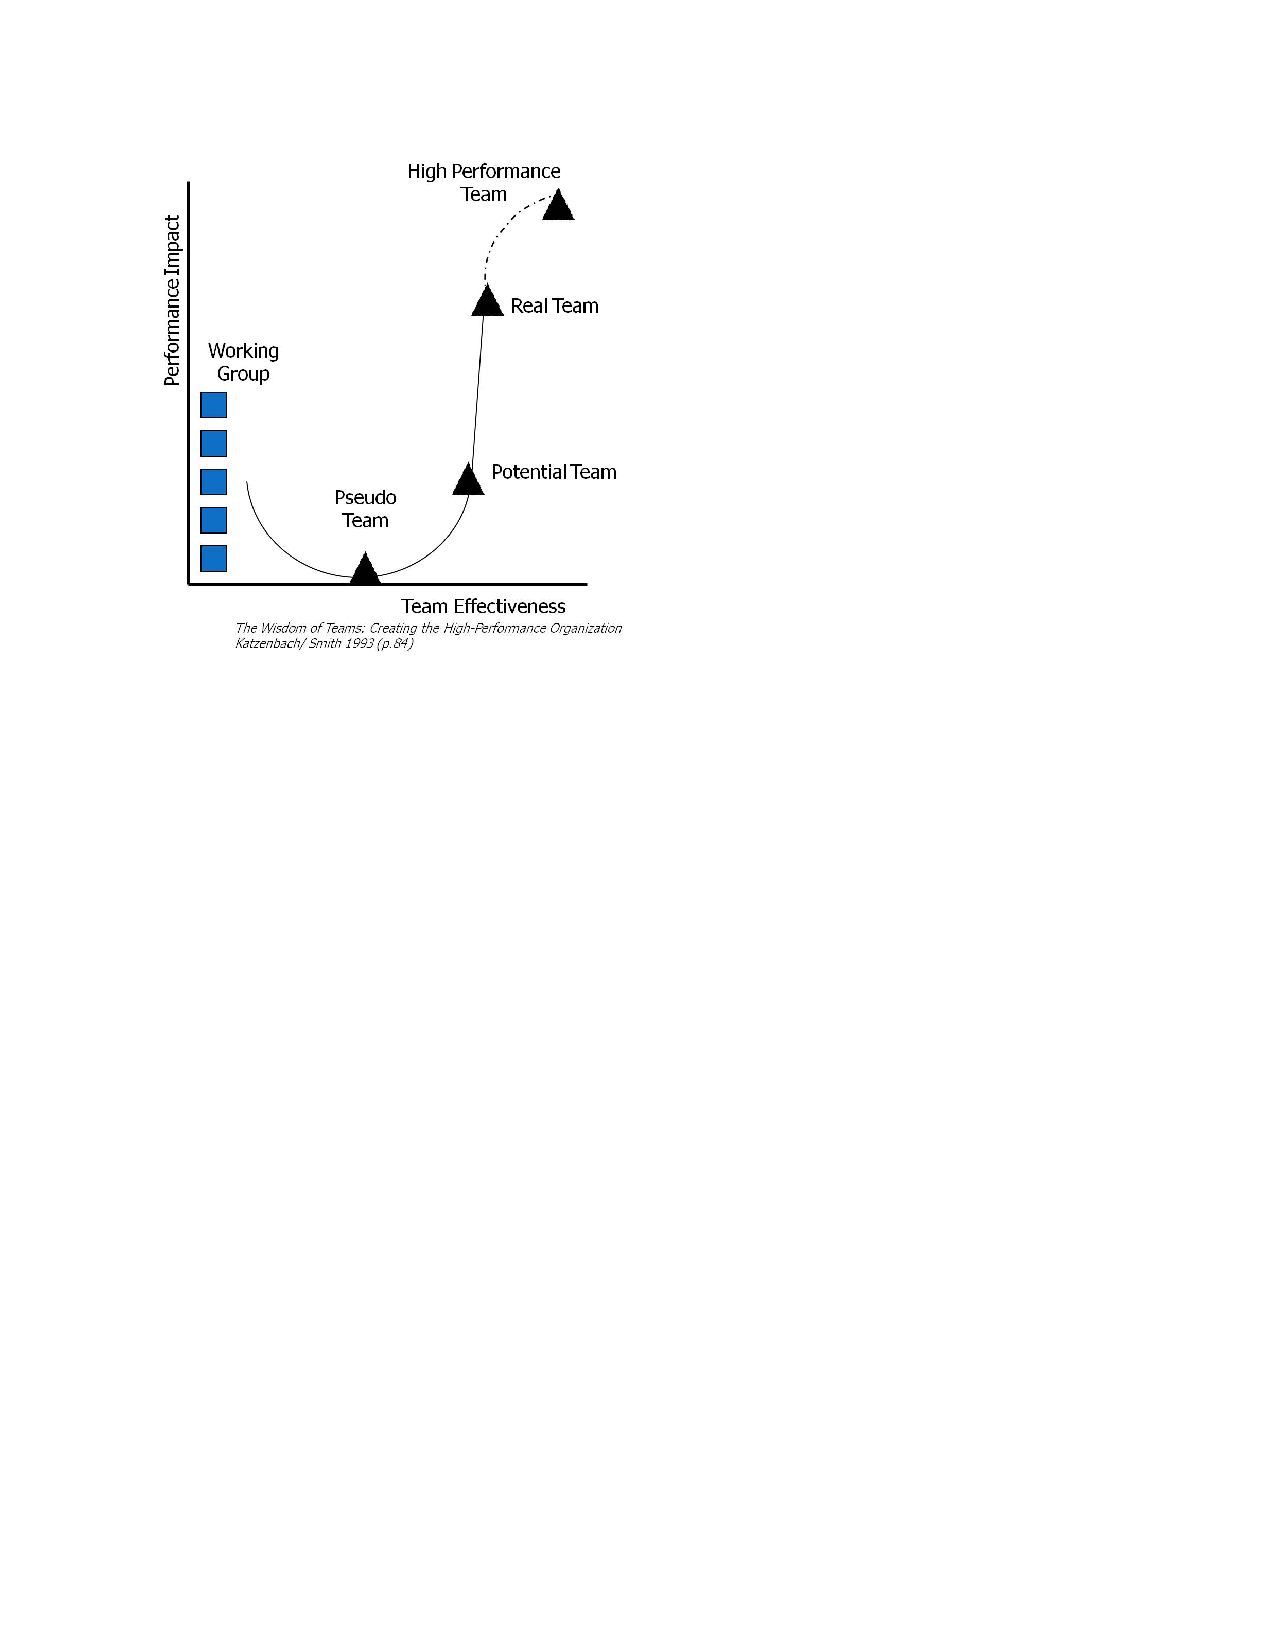
\includegraphics[clip=true, width=1 \textwidth,
trim=0cm 16cm 4cm 2cm]{Gruppetypene.pdf}
\captionof{figure}{De ulike gruppetypene}
\label{fig:gruppetype}
\end{center}

\end{enumerate}

Basert på disse karakteristikkene konkluderer vi med at vår gruppe kan karakteriseres som en effektiv gruppe. Vi er alle tilfredse og fornøyde med å arbeide sammen i en gruppe. Dessuten bidrar en felles karakter til gjensidig avhengighet og et insentiv for at alle bidrar for å oppnå et best mulig fellesresultat. Vi har regelmessige refleksjoner der vi vurderer vår egen fremdrift og effektivitet. Grunnet mangel på svært sterke emosjonelle bånd kan vi ikke definere oss som en ``high-performance"-gruppe selv om det er god stemning og vi alle etterstreber et best mulig fellesresultat. Det er ikke naturlig å forvente dette gruppetypenivået for vår gruppe da vi har svært begrenset med tid over en avgrenset tidsperiode på noen uker.\\

\section{Enighet}
\label{sec:enighet}
Enigheten i gruppa har generelt sett vært stor. Vi kan peke på flere faktorer som vi mener kan være årsaker til stor enighet innad i gruppa. I Schwarz (2002) \cite{fasilitator} sin tredje grunnregel for effektive grupper fokuseres det på at gruppemedlemmer må bruke spesifikke eksempler og bli enige om hva viktige ord og begreper betyr. Dette er et område vår gruppe har fokusert på fra første dag. Vi har vært svært opptatt av at alle har en felles forståelse av det vi diskuterer slik at man unngår misforståelser. Dette har vi oppnådd ved at alle parter, både formidler og mottaker av informasjon, til enhver tid har stilt spørsmål for å forsikre seg om at de forstår hverandre. I arbeid med utforming av tabeller til databasen hadde vi en situasjon mellom Mats og Linn som fint illustrerer dette poenget.\\

\textit{``Mats holdt på å skissere ER-diagrammet til databasen da Linn bryter inn: `det der blir vel snarere et klassediagram, jeg tror vi må gjøre det sånn her'. Linn starter å tegne sin versjon av ER-diagrammet på tavla. Mats følger litt forvirret med på Linns skisse og da hun har fått frem poenget spør han `hva er det egentlig som blir forskjellen, kan du forklare det litt nærmere Linn?' Linn forklarer hva hun mener slik at det ender med at begge er enige og oppnår en felles forståelse av de brukte ordene og begrepene."}\\

Denne situasjonen bekrefter at det er viktig med oppklaringer underveis i diskusjoner for å bli enige på samme grunnlag. Dette fokuset har trolig medført at gruppa har opplevd større grad av enighet siden misforståelser er oppdaget på et tidlig tidspunkt.\\

Samarbeidsavtalen og like bakgrunner kan være andre årsaker til stor enighet i gruppa. Store deler av dag tre ble brukt til å skrive en samarbeidsavtale. I denne forbindelse var det mye diskusjoner om hva våre ambisjoner for faget var, og hvordan vi ønsket å jobbe. Gjennom denne diskusjonen ble ønskede arbeidsforhold dokumentert slik at disse punktene lå i underbevisstheten vår under hele arbeidsprosessen. Det er mulig å anta at dette kan ha påvirket enigheten i gruppa siden vi dannet en felles plattform for hvordan vi så for oss prosjektet. På denne måten baserer alle sine meninger til dels på allerede felles prinsipper. Det faktum at vi alle har relativt like bakgrunner med tanke på utdanning og alder bidrar nok også mye til stor enighet. Vi har alle en teknisk ingeniørbakgrunn og liker struktur og bestemte måter å jobbe på. Lik utdanning og alder bidrar også til at vi oppfatter problemer på samme måte, i tillegg til å ofte se de samme løsningene.\\

Enighet i gruppa er på mange måter positivt da man unngår ubehagelige problemer og konflikter, og arbeidsprosessen går smidig og uten store hindringer. Likevel kan for stor enighet medføre at man ikke oppnår det best mulige resultatet \cite{effectiveTeams}. Denne faren kan oppstå fordi gruppemedlemmer er redd for å skape uenigheter i en ellers samlet gruppa og dermed ødelegge en god atmosfære. Dette potensielle problemet har vi forsøkt å unngå ved å følge retningslinje seks presentert av Johnson \& Johnson (2013)\cite{gruppeteori} i ``Creating effective teams": ``engasjer deg i konstruktiv kontrovers ved å være uenig og utfordre hverandres konklusjoner og resonnementer slik at kreativ beslutningstaking og problemløsning fremmes." Retningslinjen er fulgt ved at vi ved rask enighet har forsøkt å stille spørsmålstegn ved vår egen løsning, for eksempel ``hva er alternative løsninger?" og ``hva er svakhetene ved vår løsning?". Dette er en metode som har fungert relativt godt siden det har gitt diskusjonene nye dimensjoner og tvunget oss til å se saken fra ulike perspektiver.\\

\section{Involvering}
\label{sec:involvering}
Som nevnt tidligere i prosessrapporten består gruppa av både ekstroverte og introverte personer. Dette var noe vi identifiserte allerede på vår første sammenkomst. Det var lettere for enkeltpersoner å ta ordet og initiativ i forbindelse med diskusjoner og oppgaver. Wheelan (2009)\cite{effectiveTeams} påstår at kommunikasjonsmønstre etableres veldig raskt i en gruppeprosess. Hun snakker også om at effektiviteten og ytelsen til en gruppe kan lide når roller og involvering av medlemmer blir ignorert. Alle medlemmer må ta ansvar for å forsikre seg at andre blir hørt og er trygge med rolleinndelingen siden dette vil øke sjansen for gruppesuksess. Verdifulle innspill og ferdigheter vil da bli brukt istedenfor å gå tapt.\\

På landsbydag to observerte en av fasilitatorene blikkontakten blant medlemmene under en gruppediskusjon. Resultatet er vist i figur ~\ref{fig:sosiogram1}. Denne bekreftet antakelsen til gruppa om at det muligens var en skjevfordeling av deltakelse i diskusjonene.\\

\begin{center}
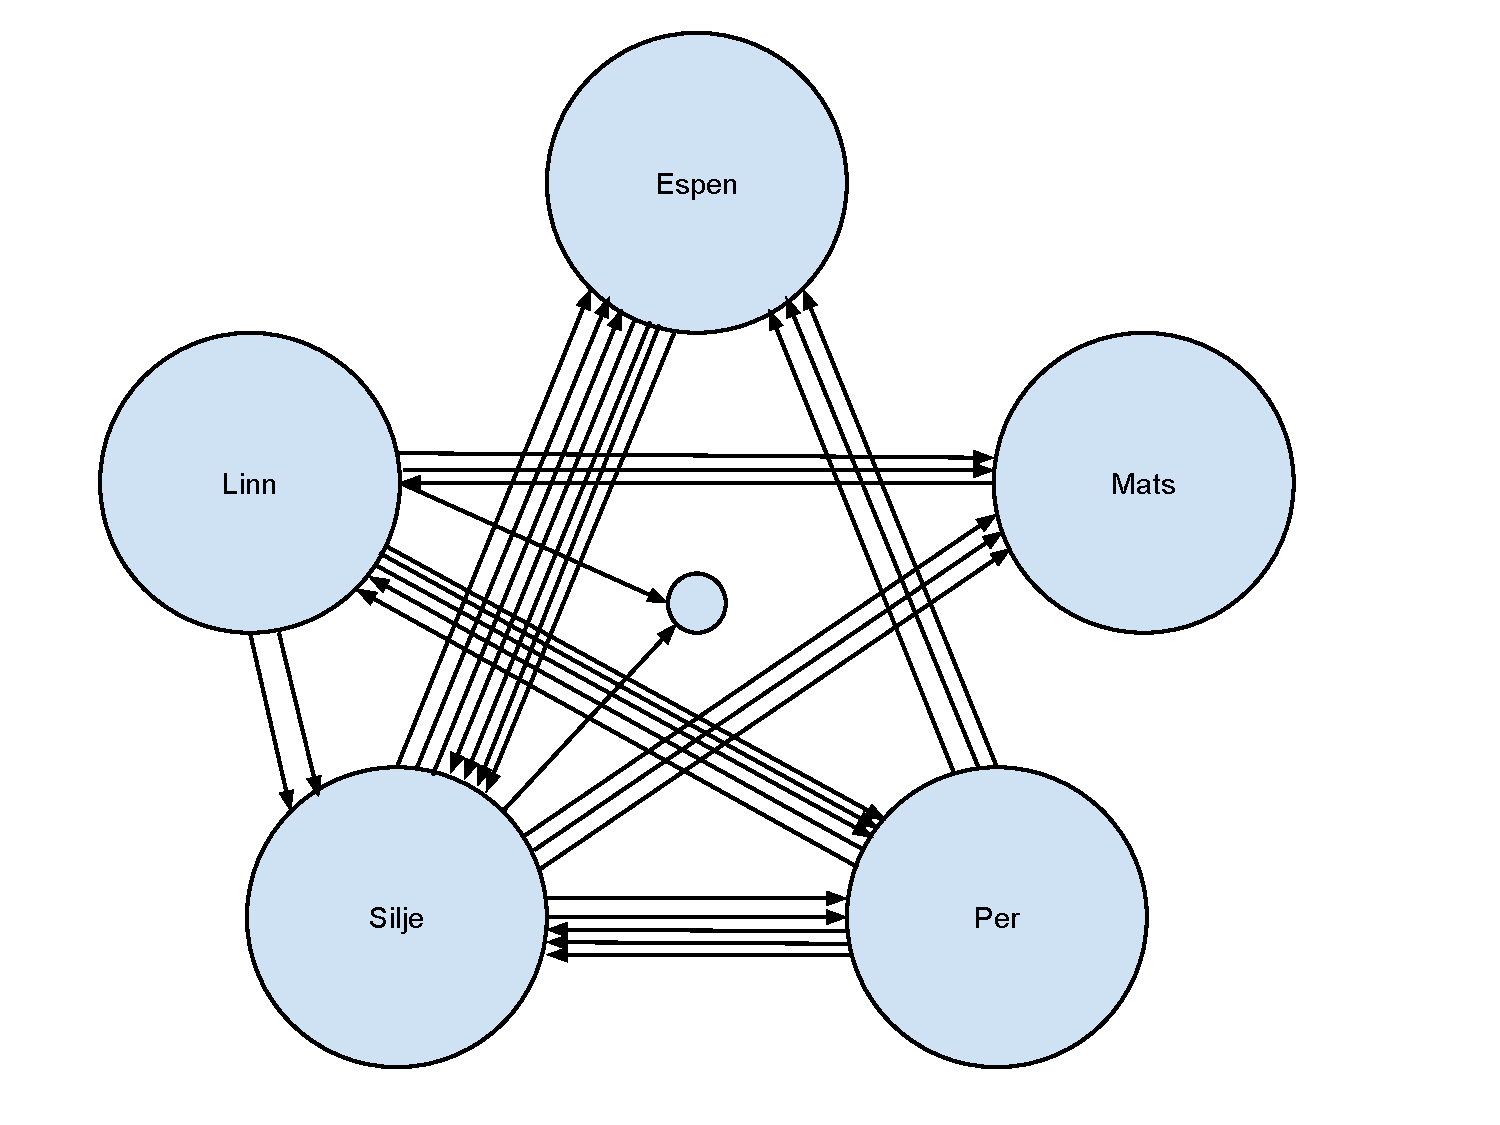
\includegraphics[clip=true, width=1 \textwidth,
trim=0cm 0cm 0cm 0cm]{Sosiogram1.pdf}
\captionof{figure}{Sosiogram 1}
\label{fig:sosiogram1}
\end{center}

I sosiogrammet over ser vi en tendens til at enkeltpersoner er mindre involvert. Man ser også antydninger til dominans fra enkeltindivider ved at mye blikkontakt er rettet mot disse. En av begrunnelsene for dette kan være at noen tar initiativet mer enn andre slik at mye fokus blir rettet mot disse personene. Et annet viktig punkt som kommer fram er at mindre fokus må rettes mot enkeltpersoner. Henvendelser må heller rettes mot hele gruppa i drøftinger. For å skape variasjon i blikkontakten i diskusjonene valgte derfor gruppa å endre sitteposisjonene seg i mellom ved jevne mellomrom. Vi håpet at dette skulle åpne opp for å lettere komme i blikkontakt med alle gruppemedlemmene i løpet av diskusjonene. Det var også viktig at alle ble observante på dilemmaet, og gjorde sitt beste for å inkludere de andre medlemmene, spesielt de som syns det er vanskeligere å ta ordet.\\

Etter de to første landsbydagene prøvde vi å sette aksjonene våre ut i praksis for å se om vi klarte å skape en plattform for deltakelse og involvering. Under arbeidet med å finne en problemstilling til prosjektet utførte vi en brainstormingprosess. Det virket som at det var en lav terskel for å komme med innspill, og vi så en omtrentlig jevn fordeling av bidragene. Espen, Linn og Silje var fortsatt partene som tok initiativet, men både Mats og Per var mer delaktige i diskusjonene. Gruppa ble enig om at det er viktig at initiativtakerne retter spørsmål og spørrende blikk mot de mer introverte partene. Dette samsvarer med Wheelan (2009)\cite{effectiveTeams} sin betraktning om at å forsikre alle sin deltakelse kan være så enkelt som å stoppe periodisk opp for å høre med alle.\\

Etter valg av tema for prosjektoppgaven skulle gruppa utarbeide en detaljert problemstilling. I den anledning foreslo Espen en uortodoks metode der hvert medlem måtte komme med et ord om gangen og dette gikk på rundgang til en fullstending problemstilling var ferdig. Dette viste seg å være en morsom og enkel måte å få alle medlemmene delaktige. Problemstillingen som ble utarbeidet viste seg også å være relativt lik den som ble brukt i selve prosjektet, noe som viste at en felles forståelse av problemet hadde blitt oppnådd ved den gode diskusjonen i brainstormingsprosessen.\\

En annen ting som ble tydelig denne dagen var at digresjoner var nyttige for å skape trygghet og trivsel i gruppa. Gruppa påpekte at det er viktig at disse digresjonene ikke tar overhånd, men at litt digresjoner skaper åpenhet innad i gruppa. Videre observerte flere at Per virket generelt mer deltakende i diskusjonene, og gruppa lurte på om dette kunne være på grunn av de tidligere aksjonene. Det var vanskelig å konkludere med at aksjonene allerede var vellykket, men gruppen valgte å se på det som et steg i riktig retning og ville fortsette med å skape en arbeidsplass hvor inkludering og trygghet var i fokus.\\

På landsbydag fire bestemte gruppa seg for å ha en overordnet rolleinndeling. I diskusjon rundt rollene virket både Mats og Per usikre på hvilken rolle de ville besitte. I den anledning bestemte Linn seg for å sette begge ovenfor et dilemma. I dette dilemmaet måtte de velge en spesifikk rolle. Dette var en god form for inkludering og skapte en sunn diskusjon som virket å skape ytterligere åpenhet mellom gruppemedlemmene. Vi ble enige om at å stille hypotetiske spørsmål kunne være en smart aksjon for å fremtvinge diskusjoner og skulle etterstrebes i høy grad.\\

Som nevnt tidligere hadde Per vist tegn til å ha følt en større trygghet i landsbydag tre, mens Mats enda hadde forholdt seg relativt stille. I landsbydag fem oppsto det dog en situasjon der Mats trådde frem. I en diskusjon rundt databasen tok han initiativ og stilte en rekke spørsmål. Det er nok flere faktorer som har innspill i denne situasjonen, eksempelvis at han føler seg mer komfortabel med å diskutere aspekter han har kunnskaper innenfor, men vi tror også at dette har med de tidligere nevnte aksjonene. De introverte gruppemedlemmene blir mer og mer delaktige, og gruppen ser en progresjon i samhold og effektivitet.\\

Et annet viktig punkt som ble observert var at enkelte av de ekstroverte personene virket å være mer observante på sin adferd. I diskusjoner prøvde disse å forholde seg mer passive for å åpne opp for at andre kunne ta initiativ og ordet. Dette er enda et tegn på gruppemedlemmenes villighet til å strebe etter et velfungerende og effektivt team gjennom inkludering.\\

I neste landsbydag jobbet Mats og Per med prototypen. I den anledning oppsto det et spørsmål vedrørende designet. Mats valgte da å forhøre seg med Silje for å få råd og meninger. Først og fremst var dette enda et tegn på at plattformen for åpenhet og inkludering vi hadde prøvd å skape virket å være vellykket. Wheelan (2009)\cite{effectiveTeams} nevner at hvis man skal dra nytte av mangfold i grupper så må alle bli involvert og hørt i diskusjoner. Selv om gruppa jobber i to subgrupper (programmering og rapportering) så er det mulig å stille spørsmål på tvers av subgruppene. En annen interessant ting var at det var en av de introverte personene som startet denne diskusjonen gjennom en rådgivning. Dette så vi på som et meget positivt tegn i forhold til oppnåelse av trygghet i gruppa.\\

Ved landsbydag åtte ble gruppa fasilitert i en av diskusjonene. Her ble diskusjon mellom de ulike partene fremstilt i et sosiogram som er illustrert i figur ~\ref{fig:sosiogram2} nedenfor. Det er viktig å poengtere at dette sosiogrammet ikke tar for seg eksakt det samme som sosiogrammet tidligere i dette delkapittelet, men omhandler i det store bildet det samme. Essensen er at begge får frem involvering i ulike diskusjoner. Det nye sosiogrammet viser helt klart forbedringer i gruppa, og vi ser en mer jevn fordeling av deltakelse. Et viktig aspekt er at både Mats og Per ikke bare henvender seg  til enkeltpersoner, men tar opp diskusjoner i hele gruppa. Det viser igjen at de introverte personene føler en større trygghet, og til og med er med på å skape involveringen selv.\\

\begin{center}
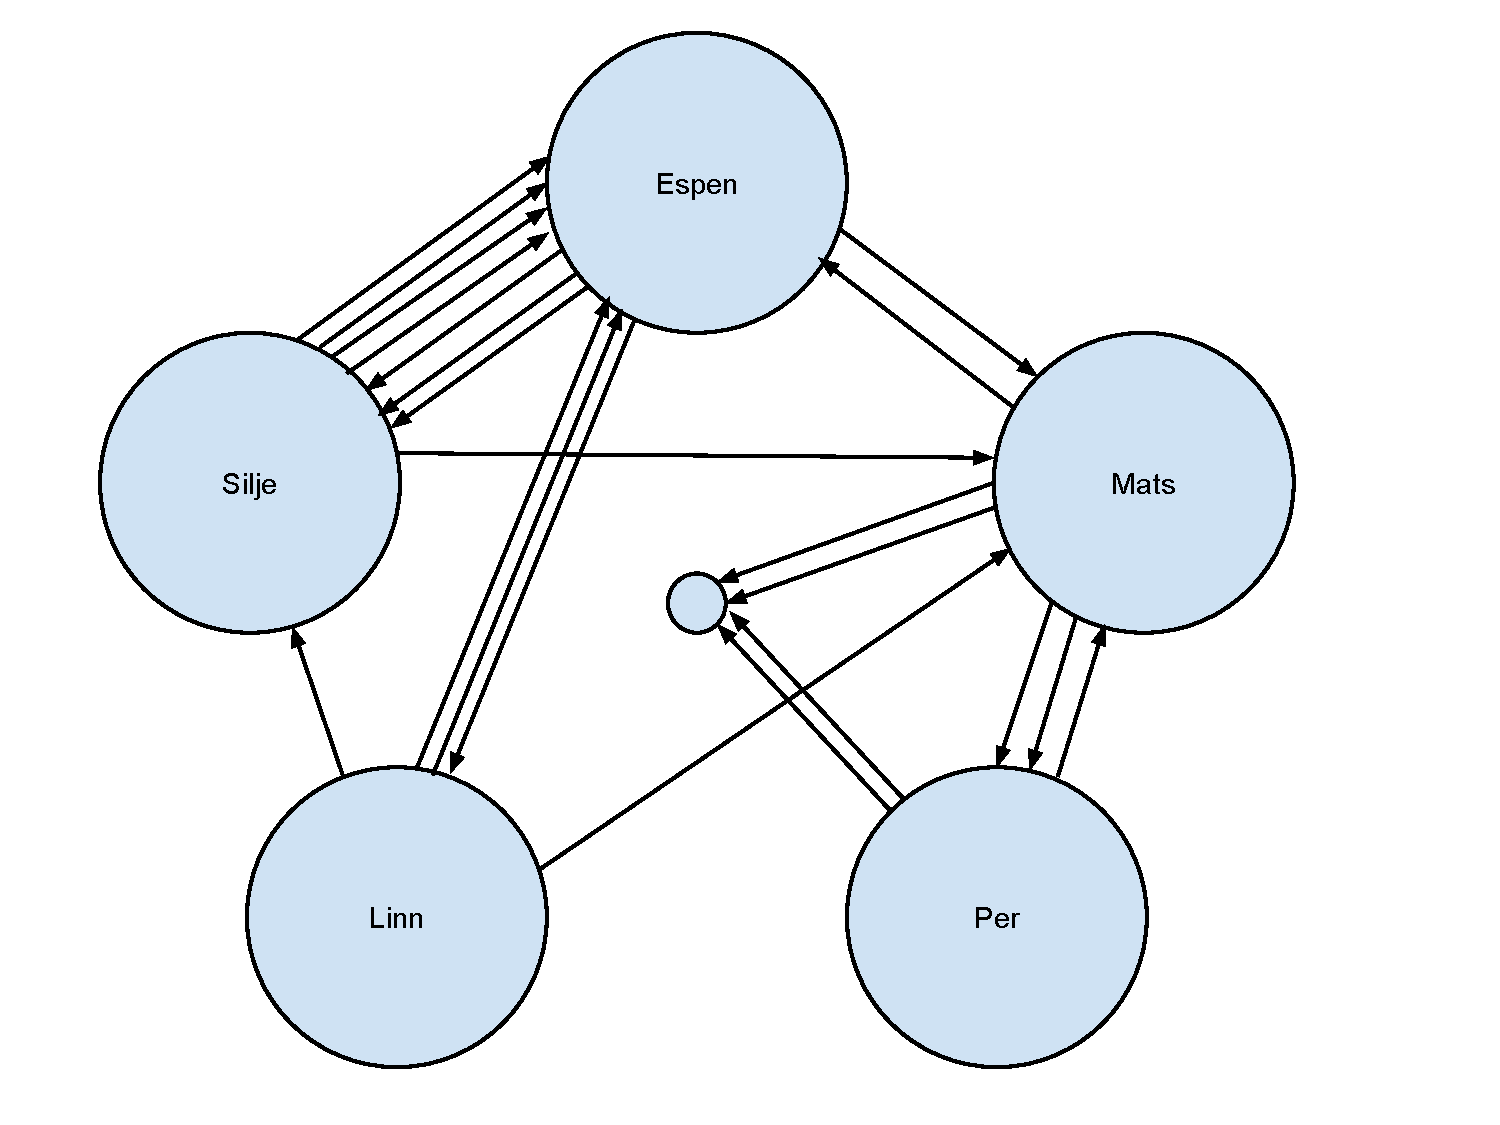
\includegraphics[clip=true, width=1 \textwidth,
trim=0cm 0cm 0cm 0cm]{Sosiogram2.pdf}
\captionof{figure}{Sosiogram 2}
\label{fig:sosiogram2}
\end{center}

En annen situasjon som oppsto på dag åtte var at Silje ved morgenmøtet lot være å ta initiativet for å gi andre muligheten. Det tyder på at de mer dominerende partene faktisk er observante på sin egen oppførsel, og er villige til å ta tak for å fremtvinge andres deltakelse.\\

I neste landsbydag kommenterte en av fasilitatorene kroppsspråket til deltakerne i en diskusjon. Han påpekte at alle var fremoverlente. En slik kroppsholdning i diskusjoner kan gjerne tyde på engasjement, og at deltakerne vil bidra med sine innspill, samtidig som de får med seg andres poenger. Observasjonen tyder på at medlemmene føler seg trygge på hverandre, og ikke er redde for å stille seg i skuddlinjen. Det er viktig at slike felles gruppediskusjoner blir brukt så ofte som mulig siden de er et godt verktøy for å videre utvikle både gruppemedlemmene på et personlig plan og gruppa som helhet.\\

Den kommende landsbydagen brakte med seg en diskusjon rundt koblingsagenten når det daglige statusmøtet ved lunsj ble utført. Fasilitatoren påpekte at alle gruppemedlemmene var delaktige i diskusjonen, og at bidragene var jevnt fordelte. Det er viktig at disse gruppediskusjonene forsetter som nevnt tidligere. Dette har ikke bare med involvering å gjøre, men også for å kunne benytte alles egenskaper og kunnskaper, samtidig som at de ulike medlemmene føler et eierskap til alle deler av prosjektet.\\

I løpet av avslutningsfasen av prosjektet så vi flere tegn på at gruppa hadde lyktes i sitt forsøk på å involvere alle i gruppa. Vi har valgt å trekke fram en spesifikk episode som vi føler gir en god indikator på dette. Ved landsbydag 11 valgte Mats å ta initiativet til oppstarten av det daglige statusmøtet etter lunsj. I en tidligere fase av prosjektet ville det vært ganske utenkelig at en av de introverte partene hadde stilt seg selv i skuddlinja, og vi anser derfor våre aksjoner som vellykkede. Alt i alt har involveringen både vært viktig for gruppas utvikling, men også for den personlige utviklingen til de ulike medlemmene.\\


\section{Beslutningstaking}
\label{sec:beslutningstaking}
I sin gruppeeffektiviseringsmodell presenterer Schwarz (2002)\cite{fasilitator} tre faktorer som bidrar til høy gruppeeffektivitet: gruppeprosessen, gruppestrukturen og gruppekonteksten. Et av punktene diskutert under gruppeprosess er beslutningstaking. I en effektiv beslutningstakingsprosess er det flere mennesker involvert . Det eksisterer en rekke beslutningstakingmetoder: konsultativ (lederen bestemmer  ved å konsultere resten av gruppa), delegerende (lederen delegerer beslutningstakingen til andre medlemmer), konsensus (beslutning oppnås når alle medlemmer kan støtte beslutningen) og demokratisk (avstemming ved flertall). Kjerneverdier ved fasilitering påstår at en gruppe er mer effektiv dersom gruppa er internt forpliktet til valgene de tar \cite{fasilitator}.\\

Basert på denne forskningen har vår gruppe valgt å strebe etter konsensus i alle beslutningstakinger, men der dette ikke lar seg gjøre skal beslutningen tas ved flertallsavstemming. Som nevnt i \ref{sec:gruppesammensetning} har vår gruppe vært preget av en stor grad av enighet slik at det stort sett har gått greit å oppnå konsensus. I beslutningen forbundet med valg av problemstilling ble konsensus vellykket gjennomført.\\

\textit{``I arbeidet med problemstillingen startet vi med brainstorming med høy grad av involvering av alle medlemmene. Deretter gikk vi gjennom hvert forslag hvor alle sa ja eller nei, ja-forslagene ble beholdt, mens nei-forslagene ble forkastet. Resultatet ble tre ideer; koblingsagent, intelligente systemer og eVoting som vi tok en inngående diskusjon av. Det ble tydelig under diskusjonen at Espen, Linn, Silje og Mats hellet i retning av koblingsagent. Per derimot var mest gira på intelligente systemer. Han fortalte at dette var et tema som interesserte han mer, og som han allerede hadde en del kunnskap om. Espen tok deretter ordet for å påpeke fordeler med å velge koblingsagenten. Han fokuserte på at vi lettere kunne benytte alle medlemmenes kunnskaper i forbindelse med en koblingsagent, i tillegg til at kompleksiteten på oppgaven var mer passende vårt tidsperspektiv. Etter litt videre diskusjon om disse faktorene, ble Per stadig mer overbevist om at koblingsagenten var et valg som ville være bra for gruppa som helhet. Vi landet derfor på en problemstilling som alle kunne stille seg bak og var motiverte for å jobbe med."}\\

Denne situasjonen ga gruppa en positiv opplevelse av konsensusmetoden. Vi erfarte at en dyptgående gjennomgang medførte at alle fikk komme med sitt syn, samtidig som gode argumenter ble presentert slik at vi dannet en felles forståelse. Dessuten unngikk vi personangrep, og diskusjonen ble drevet videre av saklige argumenter. Alle disse poengene har ligget i underbevisstheten vår i det videre prosjektarbeidet. Dette, i tillegg til at konsensus som primær beslutningsmetode ble nevnt i samarbeidsavtalen, kan ses på som aksjoner vi har gjennomført for å fortsette den gode opplevelsen av konsensusmetoden i beslutningssituasjoner.\\


\section{Samarbeidsindikator}
\label{sec:samarbeidsindikator}
%FIX X OG XX
I løpet av prosjektfasen ble det avholdt to relativt like spørreundersøkelser, henholdsvis på dag fem og ti. Disse førte med seg en samarbeidsindikator hver illustrert som pentagram i appendix \ref{appendix:samarbeidsindikator1} og \ref{appendix:samarbeidsindikator2}. Det er viktig å poengtere at den første spørreundersøkelsen ble utført av alle fem gruppemedlemmene, mens den andre bare ble gjennomført av fire slik at resultatene ikke kan sammenlignes med fullstendig nøyaktighet. Pentagrammene fremstiller fem kategorier av samarbeid, og disse vil bli videre reflektert over i avsnittet.\\

Den første kategorien omhandler i hvilken grad gruppas medlemmer forholder seg til hverandre på et personlig og direkte plan. Schwarz (2002)\cite{fasilitator} får frem at det er viktig at medlemmer er direkte med hverandre, og ikke trenger å bruke en mellommann, for å forsikre seg om at at meningene deres blir oppfattet som tilsiktet. Han nevner videre at gruppemedlemmer må kunne uttrykke seg personlig og direkte uansett hvilken posisjon eller status de har i gruppa. Hvis vi ser på samarbeidsindikatorene kan man se en minimal forbedring, og ligger ikke i en faresone.\\

Det andre feltet fokuserer på hvordan gruppa forholder seg til hverandre og det som skjer innad. Johnson \& Johnson (2013)\cite{gruppeteori} diskuterer fire ulike gruppetyper. I avsnitt \ref{sec:gruppetype} konkluderer vi med at gruppen vår tilhører kategorien ``effektive grupper". Dette kommer mye av at man føler en gjensidig avhengighet av hverandre, og er fokusert på å være oppdatert på andres arbeid. Dette blir også gjenspeilt i bruken av statusmøter i løpet av arbeidsdagene. I pentagrammene ser vi en forbedring på dette punktet. En av årsakene kan være innføringen av de nevnte statusmøtene.\\

I den tredje kategorien blir graden av snillhet og forsiktighet mellom gruppas medlemmer fremstilt. I følge pentagrammet ser vi en kraftig tilbakegang på dette punktet, og ligger i området for en stor utfordring. En av karakteristikkene ved samarbeidsgrupper er mer effektiv kommunikasjon og en vennligere atmosfære \cite{fasilitator}. Dette er en av grunnene til at vi mener det nødvendigvis ikke trenger å være direkte negativt at gruppen har skapt en mer vennlig atmosfære, og at dette kan ha bidratt til å oppnå en mer effektiv gruppe. Wheelan (2009)\cite{effectiveTeams} nevner også en vennligere gruppeatmosfære som et positivt punkt, og trekker videre fram konformitet som et positivt aspekt for samhold i grupper, noe som en vennligere atmosfære kan føre med seg.\\

Det fjerde aspektet samarbeidsindikatorene tar for seg er i hvilken grad gruppa er preget av lite struktur og svak disiplin. Schwarz (2002)\cite{fasilitator} lister opp åtte punkter som er viktige for en god gruppestruktur. Mange av disse omhandler måloppnåelse og visjoner, noe som vår gruppe har sett store likheter innenfor. Det er derfor ikke overraskende at pentagrammene viser at gruppa ikke ligger i faresonen.\\

% sjekke avsnitt 2.2.. om det er riktig referanse.
Den siste kategorien omhandler gruppas grad av asymmetri og isolasjon. Dette er noe som har blitt reflektert over flere steder i prosessrapporten (spesielt avsnitt 2.2), og har vært et stort fokus for gruppa. Samarbeidsindikatorene viser at vi plasserer oss på samme sted i pentagrammene begge ganger. Etter en refleksjon mellom gruppas medlemmer virket det veldig naturlig at vi blir plassert såpass langt ut på skalaen, men føler ikke at det trenger å være en stor utfordring. Gruppa har vært observante på fenomenet fra oppstarten, og har prøvd å snu asymetrien til en styrke der de introverte og ekstroverte partene får brukt alle sine egenskaper.\\


\section{Utvikling i løpet av prosjektperioden}
\label{sec:utvikling}
I gruppedynamikk snakker man gjerne om Tuckman sine stadier for gruppeutvikling. Denne teorien diskuterer fire spesifikke faser som er nødvendig for en gruppe for å oppnå fremgang og for å ta tak i utfordringer på en god måte. Disse fire fasene er: ``Forming", ``Storming", ``Norming" og ``Performing". Vi har valgt å ta utgangspunkt i denne teorien for å fremstille vår utvikling i løpet av prosjektfasen. De ulike fasene er illustrert i figur ~\ref{fig:faserigruppesamarbeid} under.\\

\begin{center}
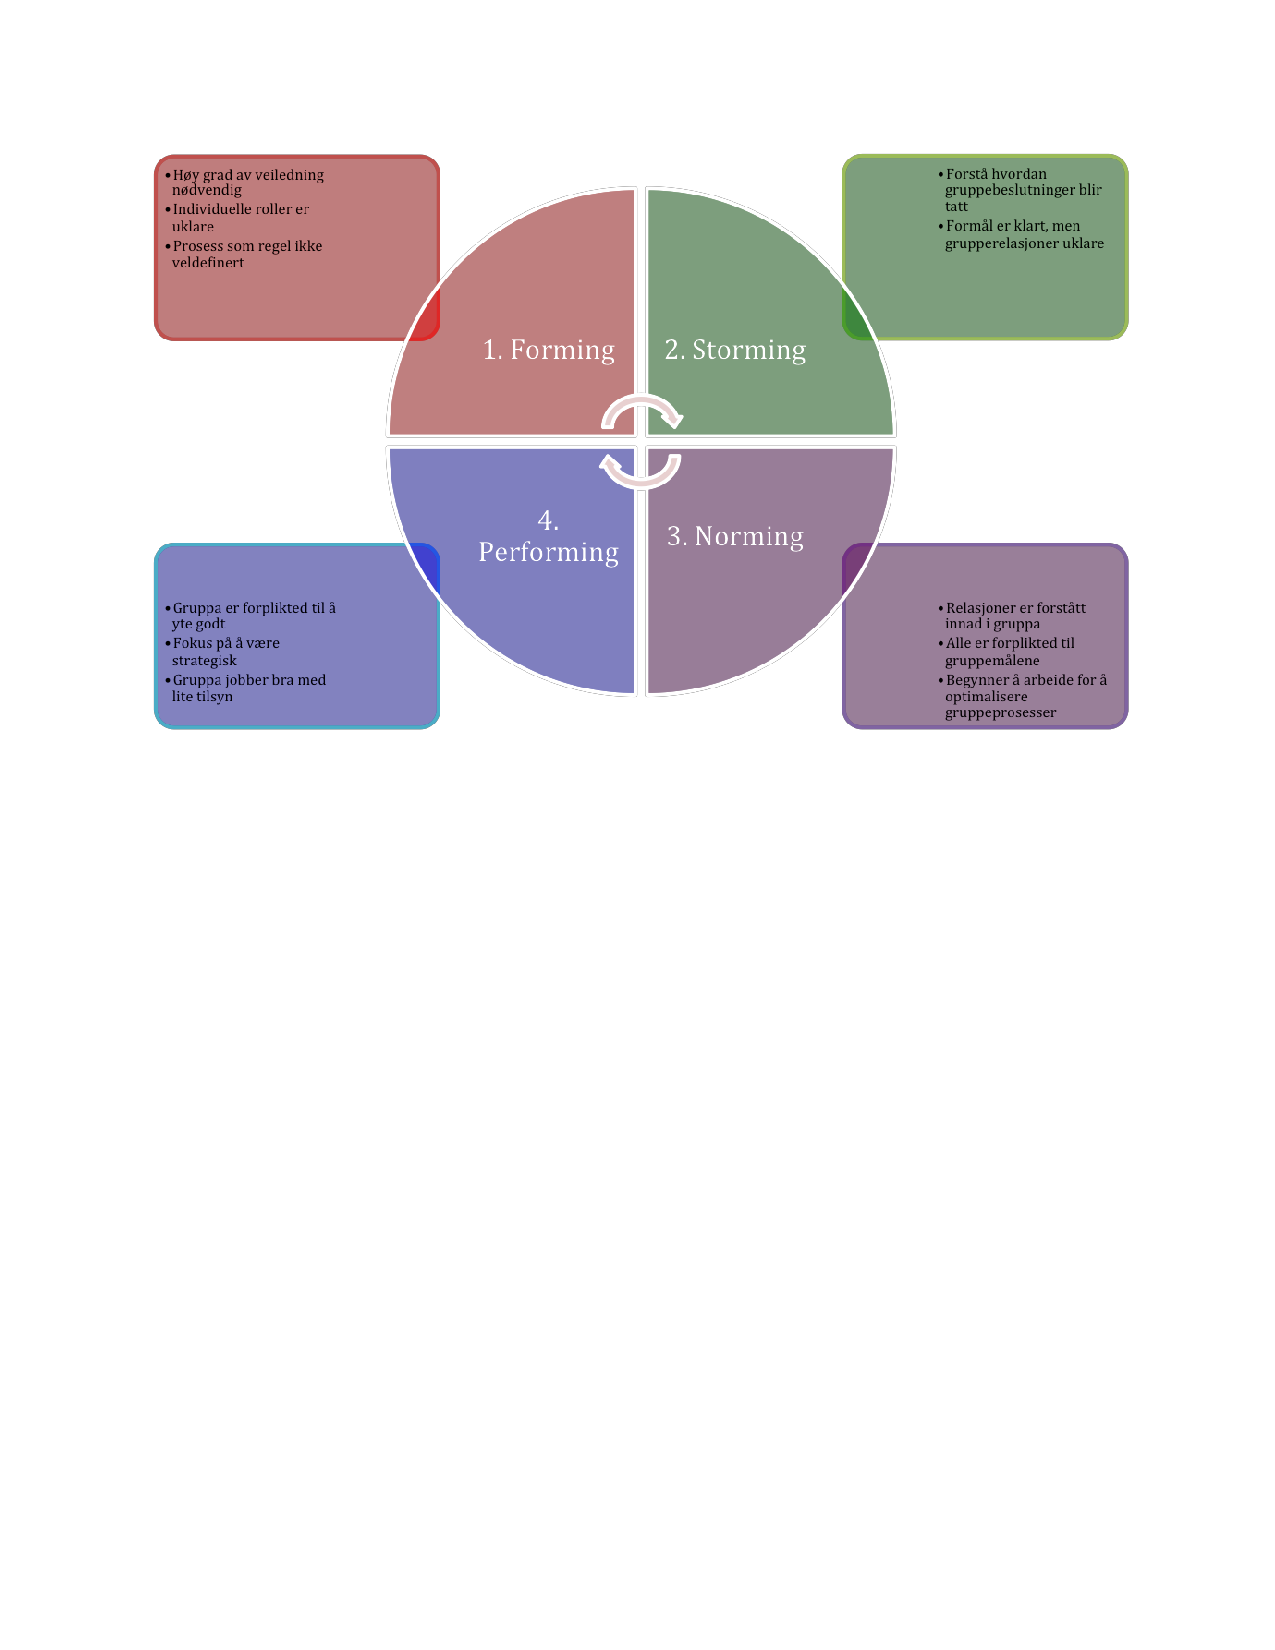
\includegraphics[scale=0.9,
trim=2.7cm 14cm 0cm 5cm]{Faserigruppesamarbeid.pdf}
\captionof{figure}{Tuckmans faser i gruppesamarbeid}
\label{fig:faserigruppesamarbeid}
\end{center}

I ``forming" fasen skal gruppemedlemmene bli kjent med hverandre. Problemer som organisering og rolleinndeling er tatt hånd om her. En annen ting som blir satt i søkelyset i denne fasen er hvordan de ulike personene arbeider individuelt, som et gruppemedlem, og hvordan de tåler press. Dette var alle faktorer som ble synlige i oppstarten av prosjektet i form av øvelsene hvor vi skulle utarbeide en kompetansetrekant og gjøre gruppa bevisst på gode og dårlige sider ved deg selv.\\

Når man avanserer fra ``forming" stadiet skal man i teorien entre ``storming" fasen. Dette var noe som ikke var like tydelig i gruppa vår. Her er det naturlig at gruppemedlemmene reflekterer og kommuniserer over sine syn, og diskusjoner blir ofte utført. Gruppa føler denne fasen omtrent ble neglisjert. Enighet rundt eksempelvis hvordan gruppebeslutninger skulle tas gikk hurtig og smertefritt.\\

``Storming" fasen var som sagt relativt kort, og ledet opp til ``norming" stadiet. I denne fasen vokste gruppa til en velfungerende enhet. Et viktig aspekt var at gruppa utarbeidet en felles plan, samtidig som felles mål og ambisjoner ble veldefinerte og fastsatt.\\

Den fjerde og siste fasen er kalt ``performing" stadiet. Det er viktig å poengtere at ikke alle grupper klarer å oppnå et slikt nivå av gruppeutvikling og gruppedynamikk. Dette er gjerne omtalt som den hellige gral i forhold til gruppeprogresjon. Gruppemedlemmene følte at vi tidlig i prosjektfasen gikk inn i denne fasen. Mye av begrunnelsen var basert på etableringen av den felles planen, målene og ambisjonene. Gruppa hadde i den anledning på et tidlig stadiet fastsatt rammene for prosjektet, og gikk dermed på skinner. En annen viktig faktor for oppnåelsen av ``performing" fasen var måten gruppa inndelte arbeidet der alle medlemmene fikk benyttet sine styrker. Effektivitetsnivået var meget høyt, som vi så på som et tegn for hvor langt gruppa hadde kommet som en enhet.\\

Som det fremgår av teksten over har gruppa faktisk gått gjennom de ulike stadiene i Tuckman sin teori om gruppeutvikling, men har omtrent forbigått ``storming" fasen. Gruppa utviklet seg til en velfungerende enhet i løpet av prosjektet. Dette kunne observeres fra flere faktorer. Eksempelvis så man en stadig økning i produksjonsnivå og effektivitet. Det var en enighet om at oppnåelsen av denne fasen var meget positiv, spesielt siden dette ikke skal tas forgitt. Det er også viktig å ta i betrakning tidsaspektet og at gruppemedlemmene hadde liten kjennskap til hverandre på forhånd.\\


\chapter{Personlig utvikling i et læringsperspektiv}
Hensikten med EiT er som nevnt tidligere å forbedre samarbeidsevnene til medlemmer i ett tverrfaglig team ved å anvende sin fagkunnskap i et prosjektarbeid. Det var næringslivet som insinuerte at studentene burde få erfaring i å samarbeide med personer med ulik fagbakgrunn enn dem selv, og at de burde få mer øvelse i å bruke sin fagkompetanse til å løse komplekse oppgaver. Erfaringslæring står i fokus i EiT og utgangspunktet for læringen skal være refleksjon over konkrete arbeidssituasjoner. (\textit{Hva er Eksperter i team (EiT)}?, 2013)\\

I følge seksjon \ref{sec:sammensetning} hadde gruppas medlemmer mye av de samme forventningene til EiT, men noen vektla visse aspekter mer enn andre. Nedenfor har gruppas medlemmer reflektert over sin personlige utvikling i løpet av prosjektprosessen, samt hvilket utbytte faget har gitt dem.\\

Linn: \textit{``Når jeg ser tilbake på EiT så har det helt klart vært en veldig positiv erfaring å ha med seg videre. Jeg synes det gikk litt tregt i starten med alle øvelsene vi skulle gjøre i plenum, men etter at vi fikk jobbe litt mer selvstendig så har jeg lært utrolig mye om det å jobbe i gruppe. Jeg har blitt mer bevisst på å tilpasse meg andre i gruppa og ser viktigheten av å gi og ta i en gruppe for at dynamikken skal bli så god som mulig. Videre så har jeg holdt på mye med det tekniske, altså programmering av PHP, javascript, HTML og CSS og føler jeg har lært en del der. Selv om det jeg har lært aller mest av er at det er viktig å reflektere over det man gjør i gruppa, snakke sammen og planlegge for å oppnå et godt resultat."}\\

Silje: \textit{``EiT har gitt meg mye ny erfaring og kunnskap. Selve arbeidet med prosjektet og koblingsagenten har medført at jeg har tilegnet meg ny terminologi innenfor tekniske områder som MySQL, PHP, Github og Javascript. Likevel er det selve prosjektprosessen som har gitt meg mest lærdom. Jeg føler at jeg har blitt mye mer bevisst på hvordan jeg oppfører meg og hvordan jeg bør oppføre meg i en gruppe for å ende opp med best mulig resultat. Det har vært veldig lærerikt med den ulike fasiliteringen fordi den har gjort oss klar over situasjoner som ellers ville gått upåaktet hen. Alt i alt har min EiT-opplevelse vært positiv, og jeg tror absolutt at faget har forbedret mine samarbeidsevner."}\\

Espen: \textit{``I løpet av prosjektets gang har jeg blitt tilført mange nye erfaringer. I hovedsak har disse erfaringene omhandlet hvordan jeg som gruppemedlem blir oppfattet av andre. I den anledning har faget gitt meg bedre selvinnsikt, og har ført til at jeg har gjort endringer for å bedre gruppa som helhet. Jeg føler også at EiT har gjort meg mer bevisst på hvordan man kan evaluere andre, og hvordan man skal fremstille disse observasjonene på en god og konstruktiv måte. Videre har faget gitt meg faglig kunnskap innenfor emner jeg ikke besatt før, spesielt relatert direkte til koblingsagenter. I sin helhet har emnet brakt med seg et meget positiv inntrykk, og jeg føler helt klart at mine opprinnelige mål har blitt oppfylt."}\\

Per: \textit{``EIT har for meg vært en positiv opplevelse, hvor jeg har lært mye om gruppedynamikk og hvilke faktorer som er viktige for at en gruppe skal fungere bra. Videre har jeg også blitt mer bevisst på hvordan andre opplever meg som et gruppemedlem og hva jeg kan gjøre for å være et best mulig gruppemedlem. Det har også vært en god leksjon i evaluering av meg selv og evaluering av andre på gruppa. Faglig har jeg fått en oppfriskning av webspråk og lært en god del om hvordan man kan skrive koblingsagenter som er kosteffektive til riktig formål, med tanke på tid det tar å utvikle, skalerbarhet, utviklingspotensial osv."}\\

Mats: \textit{``I utgangspunktet var jeg noe skeptisk til EiT og opplegget, basert på hva jeg hadde hørt fra andre, og det generelle førsteinntrykket jeg fikk. Dette viste seg fort å være ubegrunnet skepsis, da jeg har opplevd opplegget som positivt. Jeg har blitt mer bevisst på hva som definerer godt gruppesamarbeid og tiltak som kan gjøres for å videre fremme samarbeid.  Selv føler jeg at jeg har hatt en personlig utvikling under EiT prosjektet, da jeg spesielt har fått noe innsikt i hvordan andre gruppemedlemmer oppfatter meg. Jeg har også fått ett noe annet syn på hvordan åpenhet kan påvirke samarbeid generelt i en positiv retning. Jeg har også lært noe av programmeringsspråket PHP, for utvikling av web-baserte applikasjoner."}\\

Basert på disse refleksjonene kan vi konkludere med at gruppemedlemmene overordnet sett har hatt et positivt inntrykk av EiT. Alle påpeker at de har fått ny, faglig innsikt, men at det er refleksjonene rundt selve prosessen som har gitt dem mest ny kunnskap. En ordsky illustrert i figur \ref{fig:Ordsky}) er generert med utgangspunkt i de personlige refleksjonene for å illustrere hva som er gjennomgående i gruppemedlemmenes refleksjoner. Ordskyen kan indikere fellestrekk i gruppemedlemmenes oppfatning av læringsutbytte i faget som igjen kan sammenliknes med fagets læremål.\\

\begin{center}
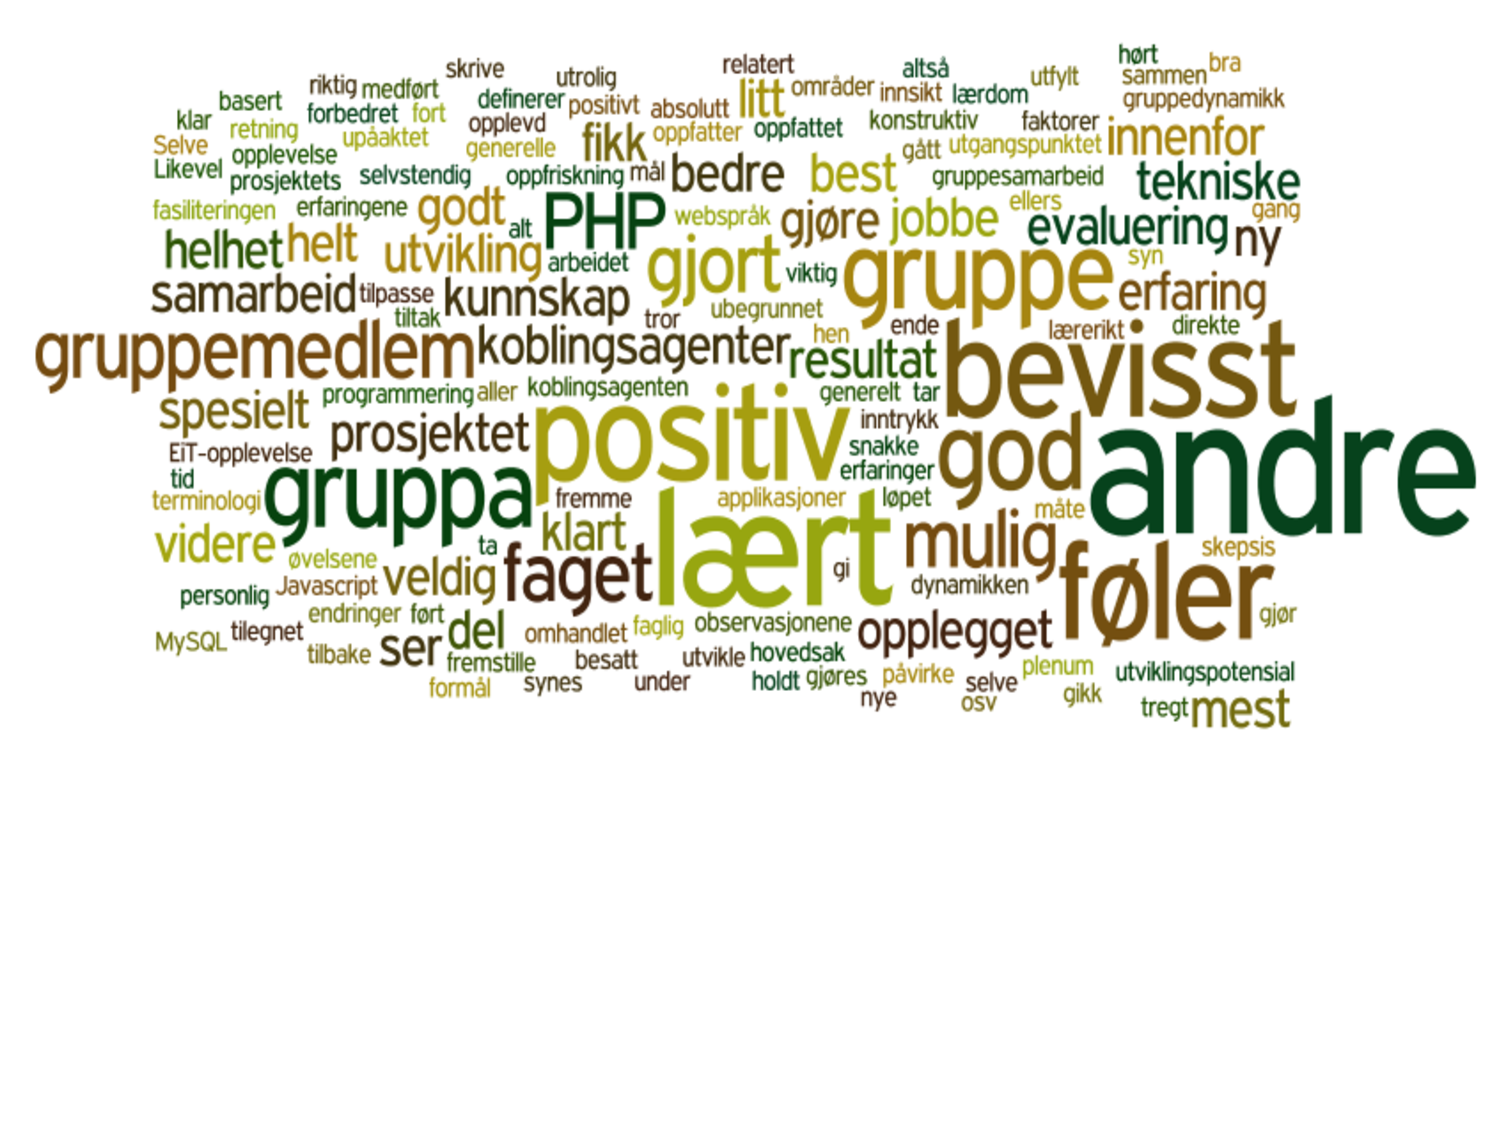
\includegraphics[clip=true, width=1 \textwidth,
trim=0cm 5.5cm 0cm 0cm]{ordsky.pdf}
\captionof{figure}{Ordsky generert av refleksjoner}
\label{fig:Ordsky}
\end{center}

Ordene \textit{andre, positiv, bevisst, gruppe/gruppa, lært, føler og PHP} skiller seg ut som noen av de mest brukte ordene. Dette resultatet bekrefter tidligere påstander om at gruppemedlemmene generelt sett har ett positivt inntrykk av EiT og at prosessen og samarbeidet har stått i sentrum. Av de åtte mest brukte ordene er det kun ett av de som omhandler den tekniske biten av arbeidet; PHP, mens mange omhandler selve samarbeidsprosessen. Spesielt ordet bevisst skiller seg ut. Dette tyder på at gruppemedlemmene føler at de har blitt mer bevisst på ulike aspekter ved gruppearbeid, noe som går igjen i flere av fagets læremål.\\

Alt i alt, kan vi konkludere med at gruppa har lært mye i løpet av prosjektperioden og flere av læremålene er tilsynelatende oppfylt.\\


\chapter{Evaluering og oppsummering}

Som en innledning til faget ble våre individuelle forventninger skrevet ned og presentert. Disse forventingene var mål og ambisjoner vi håpet på å oppfylle i løpet av prosjektfasen, og som alle medlemmene har etterstrebet. På slutten av prosjektet valgte gruppen å analysere utbytte av faget, og om de ulike målene og ambisjonene var oppnådd. I kapittel 4 er dette presentert grundig der alle medlemmene satt igjen med et godt inntrykk av opplevelsen EiT hadde brakt med seg. Mer spesifikt så man klare likhetstrekk mellom de individuelle analysene der alle gruppemedlemmene virket å ha blitt mer bevisst på ulike aspekter ved gruppesamarbeid.\\

Prosjektet førte også med seg ulike situasjoner i løpet av arbeidsfasen. Disse ble hovedsakelig oppdaget ved hjelp av personlige refleksjoner og grupperefleksjoner. De mest markante situasjonene var enighet, involvering og beslutningstaking, og er henholdsvis diskutert i avsnitt 3.2, 3.3 og 3.4. Alle situasjonene har vært tilstedeværende i løpet av hele prosjektets gang, og har vært områder gruppemedlemmene og gruppa som helhet har satt mye fokus på. De ulike situasjonene har vært i konstant utvikling, der ulike aksjoner utført av gruppa har drevet situasjonene i en positiv retning, og har styrket både samhold og kvalitet på det endelige arbeidet. De ulike situasjonene har også økt bevisstheten innenfor disse spesifikke områdene til de forskjellige gruppemedlemmene.\\

Mye av prosessrapporten har fokusert på gruppas utvikling, både som helhet og på det individuelle planet. Gruppemedlemmene har gjennomført både personlige refleksjoner og grupperefleksjoner som har blitt benyttet til å analysere spesifikke hendelser, og har vært grunnlaget bak ulike tiltak. Mange av disse tiltakene har resultert i forbedringer av gruppas arbeidsmetoder, og har bidratt til økt selvinnsikt. Emnebeskrivelsen og emnets læringsmål nevner at faget skal bidra økt innsikt og utvikling av gruppemedlemmenes samarbeidsevner. Dette er noe alle medlemmene føler faget har ført med seg, og som framtidige arbeidstakere føler vi oss mer utrustet i forhold til senere prosjektarbeid i det tverrfaglige yrkeslivet.


\newpage
\appendix
\addcontentsline{toc}{chapter}{Appendix}
\chapter{Samarbeidsavtale}
\section{Samarbeidsavtale}
\label{appendix:samarbeidsavtale}
\bf{Gruppe 2 - ''IT for en bedre verden''}\\

\bf{\textit{Leveranse}}
\begin{enumerate}
\item Gruppa er enige om at alle skal bidra tilnærmet likt i arbeidet med både prosess- og prosjektrapport. Vi vil ha en overordnet ansvarlig for henholdsvis prosess- og prosjektrapporten, men alle på gruppa skal etterstrebe at rapportene er av en slik kvalitet at de tilfredsstiller kravene til en toppkarakter (A/B).
\item Alle møter til avtalt tid. Skjer det noe spesielt så skal det gis beskjed snarest mulig til hele gruppa på telefon eller Facebook om forsinkelser eller fravær. Ved mangel av beskjed blir dette tatt opp ved neste møte.
\item Etter innsjekk hver landsbydag har gruppa en “daily standup” for å kartlegge hva som er blitt gjort siden sist og sette opp mål for dagen.
\item Det forventes at alle gjør arbeidet som de har blitt tildelt til gitte tidsfrister.\\


\bf{\textit{Trivsel}}

\item Gruppa ønsker å skape en plattform for åpenhet og inkludering hvor alle har en lik mulighet til å komme med innspill.
\item For å sikre en effektiv arbeidsdag hvor motivasjonen holdes oppe så ønsker gruppa å ha effektive arbeidsøkter på ca 1 time avbrutt av en ca 5 minutters pause. I disse arbeidsperiodene skal mobiler legges vekk slik at fokuset blir opprettholdt.
\item Vi setter opp milepæler underveis i fremdriftsplanen hvor alle har ansvar for å utføre sin del av arbeidet til gitt milepæl. Gjennomført milepæl symboliseres.
\item Ved oppdagelse av avvik eller uenigheter skal dette tas opp på et tidligst mulig tidspunkt for å unngå at problemet eskalerer.
\item Dersom en konflikt går ut av kontroll skal fasilitator kontaktes for rådgivning.
Ved beslutninger skal kompromiss etterstrebes. Der dette ikke lar seg gjøres benyttes avstemning.\\

\bf{\textit{Læring}}

\item Under møter og diskusjoner så rulleres det på sekretærrollen slik at alle bidrar likt jevnt over alle møter og diskusjoner.

\item Det er viktig at man stiller (kritiske) spørsmål selv om en eller flere personer viser høy kompetanse innenfor emnet. Dette for å øke bevisstheten og kunnskapen til alle i gruppa.

\item Ved tilførsel av ny kunnskap skal man forsikre seg om at alle gruppemedlemmene er underforstått med innholdet, at det er entydig.
\end{enumerate}

\chapter{Samarbeidsindikatorer}
\section{Samarbeidsindikator 1}
\label{appendix:samarbeidsindikator1}

\begin{center}
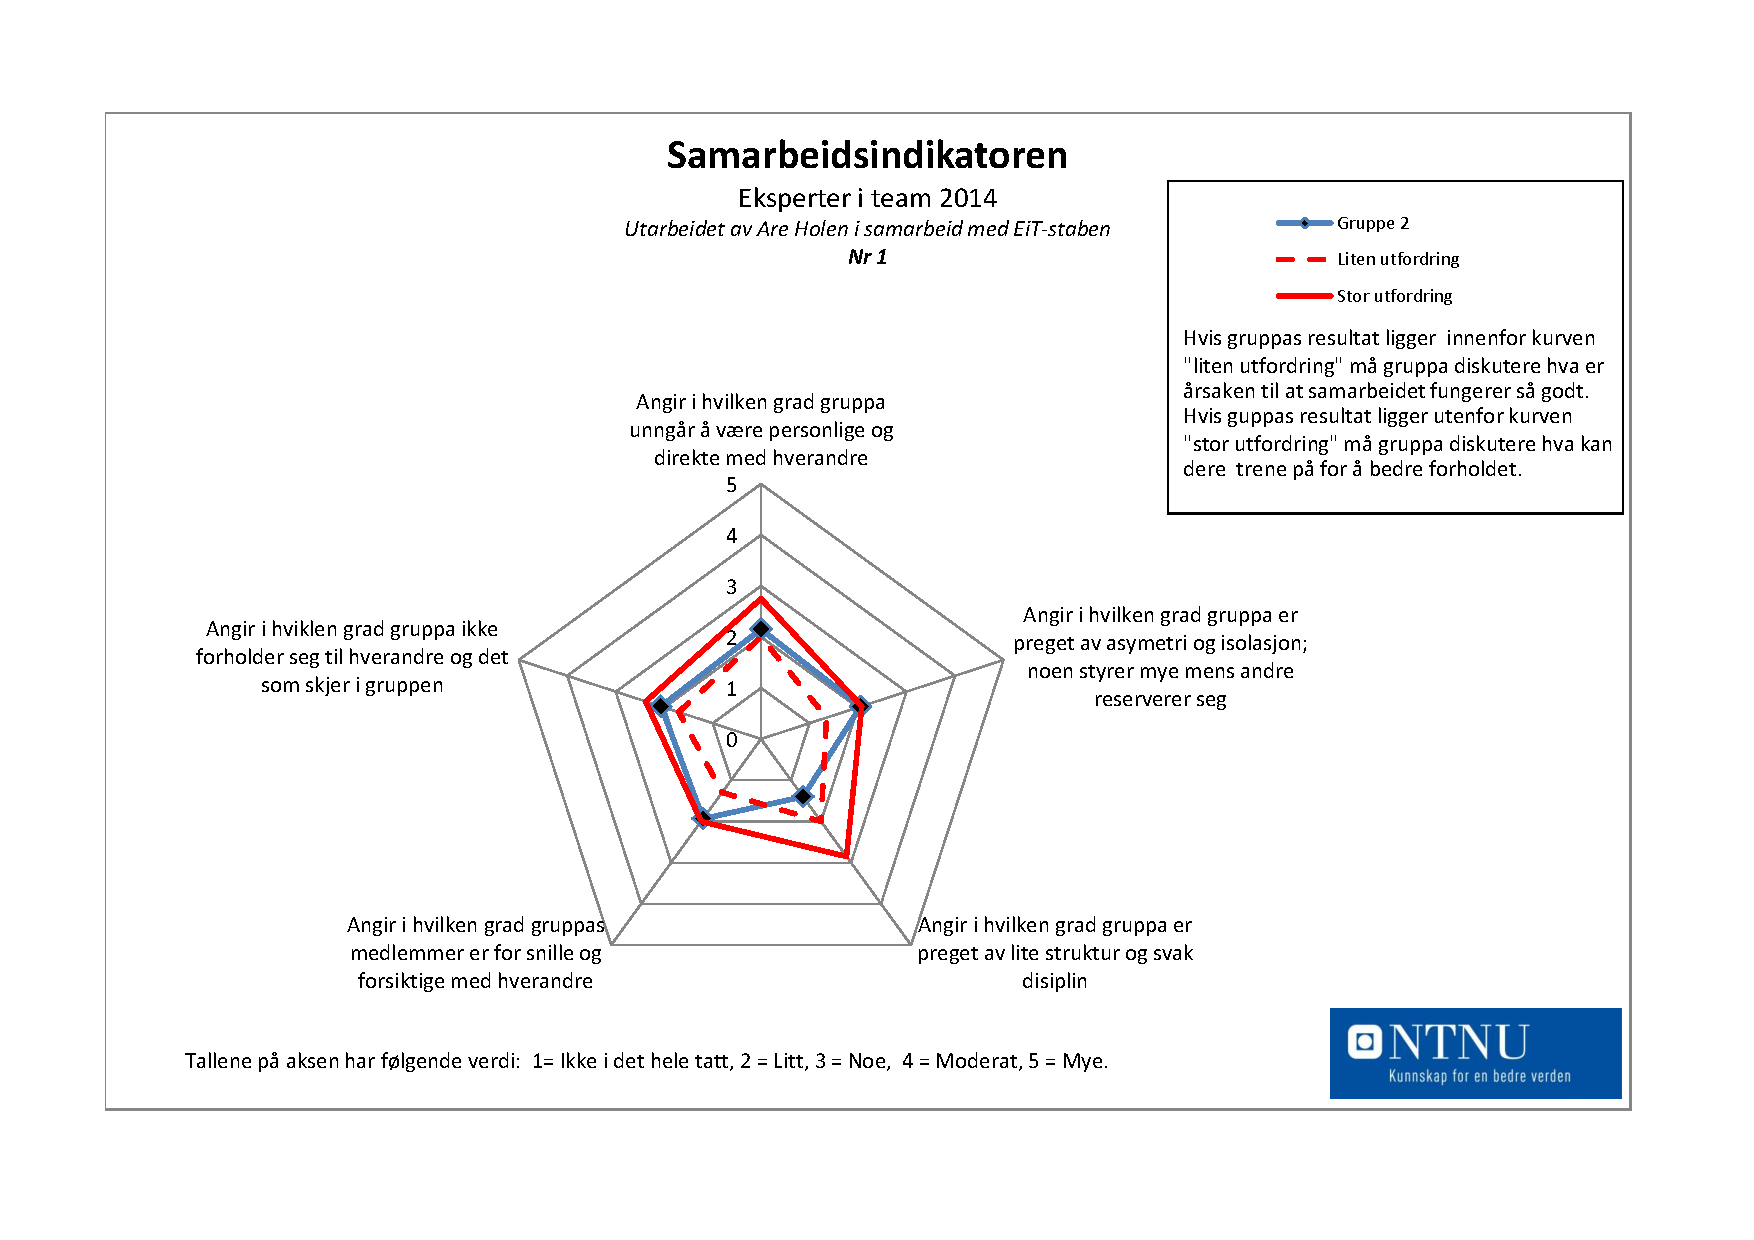
\includegraphics[clip=true, width=1 \textwidth,
trim=0cm 0cm 0cm 0cm]{Samarbeidsindikator1.pdf}
\captionof{figure}{Samarbeidsindikator nr.1}
\label{fig:indikator1}
\end{center}

\section{Samarbeidsindikator 2}
\label{appendix:samarbeidsindikator2}
\begin{center}
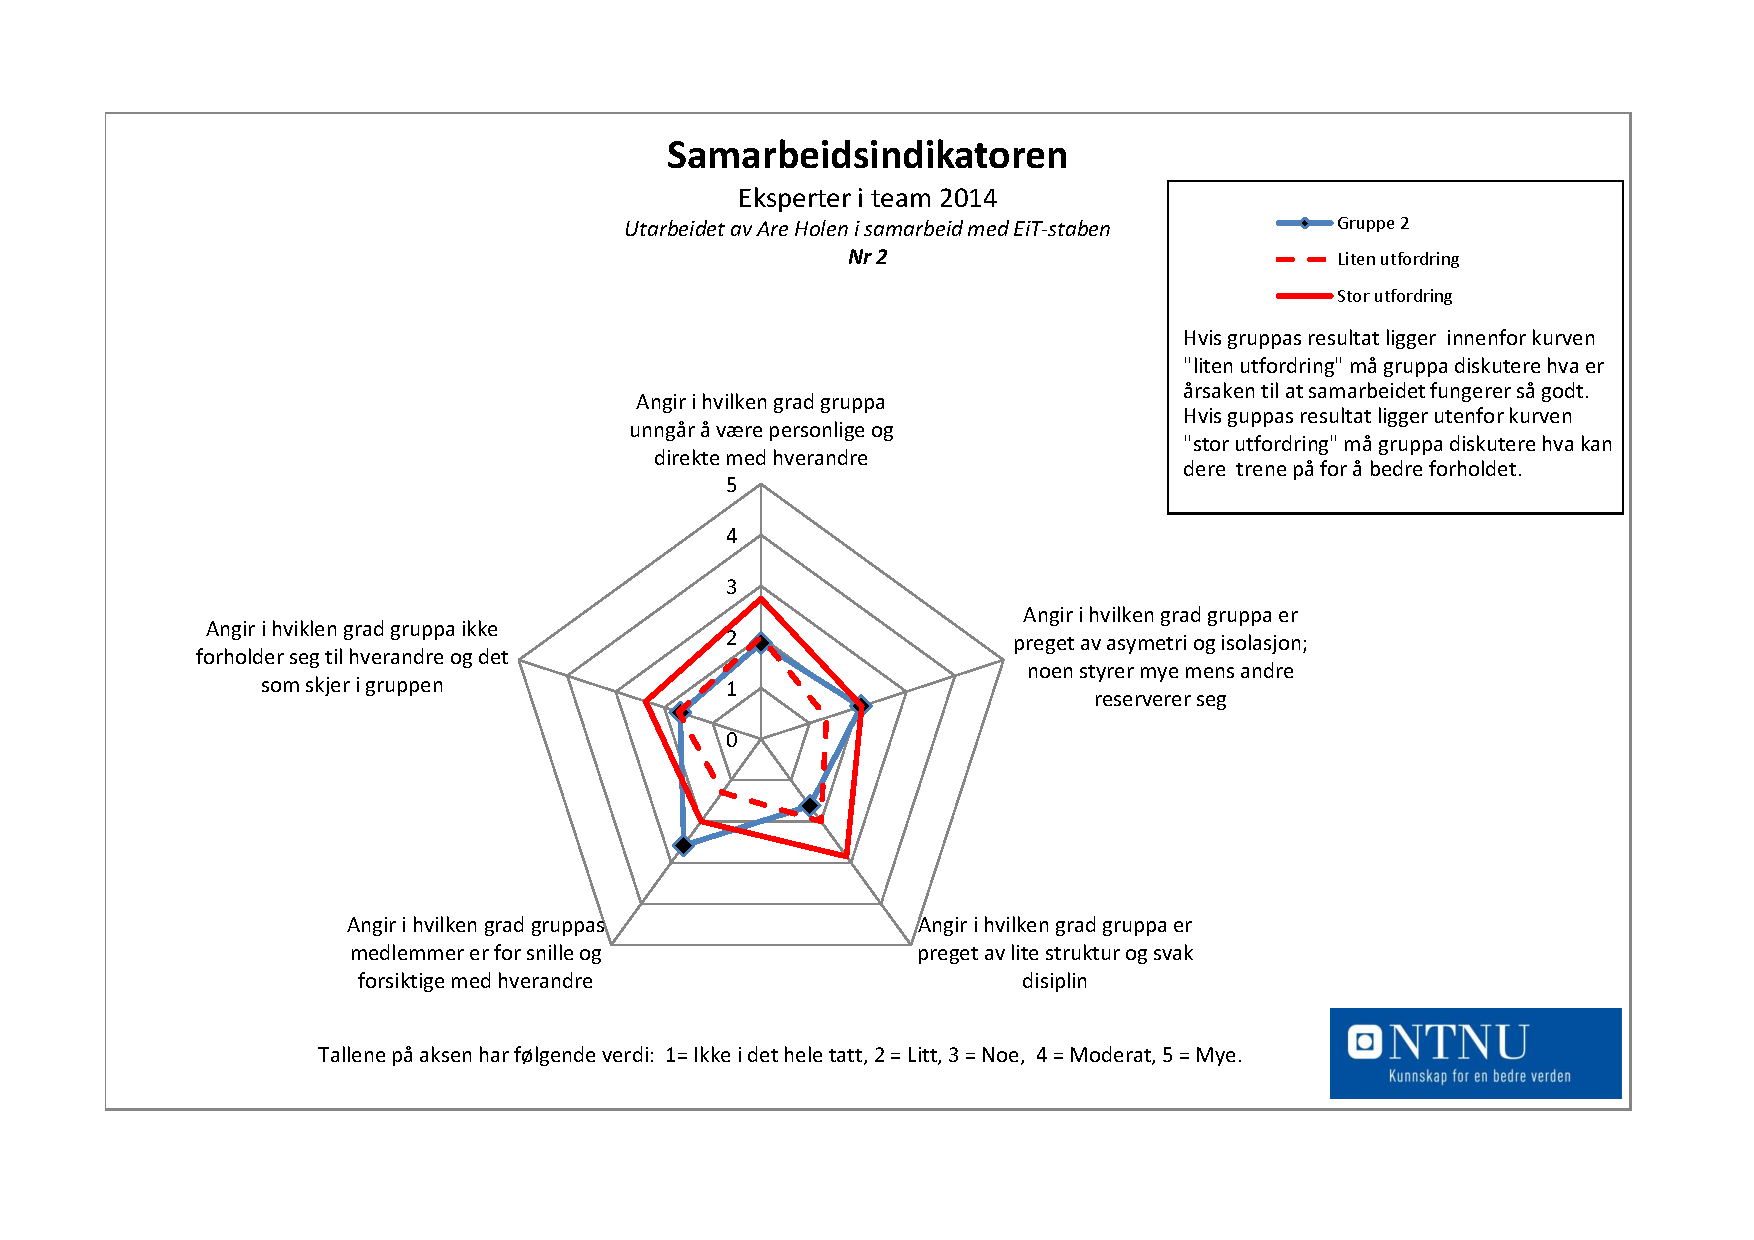
\includegraphics[clip=true, width=1 \textwidth,
trim=0cm 0cm 0cm 0cm]{Samarbeidsindikator2.pdf}
\captionof{figure}{Samarbeidsindikator nr.2}
\label{fig:indikator1}
\end{center}


\bibliographystyle{plain}
\bibliography{bibl}
\end{document}
